\documentclass[11pt,a4paper]{article}

\usepackage[margin=2.2cm]{geometry}
\usepackage[T1]{fontenc}
\usepackage{lmodern}
\usepackage{amsmath,amssymb}
\usepackage{graphicx}
\usepackage{booktabs}
\usepackage{tabularx}
\usepackage{array}
\usepackage{float}
\usepackage{caption}
\usepackage{subcaption}
\usepackage{xcolor}
\usepackage{enumitem}
\usepackage{tikz}
\usetikzlibrary{arrows.meta,positioning,fit,calc}
\usepackage[siunitx]{circuitikz}
\usepackage[colorlinks=true,linkcolor=blue!50!black,urlcolor=blue!60!black,citecolor=blue!50!black]{hyperref}

\graphicspath{{figures/}{figures/screens/}}
\setlength{\parskip}{4pt}
\setlength{\parindent}{0pt}
\captionsetup{font=small,labelfont=bf}
\renewcommand{\arraystretch}{1.12}
\newcommand{\code}[1]{\texttt{\small #1}}
\newcommand{\pct}{\,\%}

\title{\textbf{ML-Driven PVT-Variation-Aware Leakage Estimation}\\[4pt]
\large Digital VLSI Design --- Course Project Report}
\author{Saumya Vira \and Anish Toshniwal \and Shrenil Patel \and Het Selarka}
\date{November 2026}

\begin{document}
\maketitle

% ------------------------------------------------------------------------------------------
\section*{Project repository}
All code, datasets, netlists, trained models, result files and this report are available at\\[3pt]
\centerline{\large\url{https://github.com/realsvira/DVD_Project}}\\[3pt]
\code{python run\_all.py -{}-mode verify} checks the environment, runs the 92 automated tests and audits all
deliverables; \code{-{}-mode full} regenerates everything from the model file with fixed seeds
(see \code{README.md} and \code{docs/INSTALL\_WINDOWS.md}).

\begin{table}[H]
\centering
\caption{Team assignment (given by the TAs).}
\begin{tabular}{ll}
\toprule
Team & Saumya Vira, Anish Toshniwal, Shrenil Patel, Het Selarka \\
Model file & \code{45nm\_HP} (PTM 45\,nm high performance, metal gate / high-k) \\
Nominal VDD & 1\,V \\
Test circuit & 3-bit carry-lookahead (CLA) adder \\
\bottomrule
\end{tabular}
\end{table}

\section*{Contributions}
The work was split into four parts of comparable size; every part was done by a pair, and every member
worked on exactly two parts, so each member contributed an equal share (25\pct).

\begin{table}[H]
\centering
\caption{Division of work.}
\small
\begin{tabularx}{\textwidth}{>{\raggedright\arraybackslash}p{4.1cm}X>{\raggedright\arraybackslash}p{3.3cm}}
\toprule
Part & Work & Members \\
\midrule
A1: Simulation engine and datasets & ngspice setup, batch simulation engine, single-transistor netlists, PVT sampling,
the four 10{,}000-sample datasets, Kirchhoff check and trend plots & Saumya Vira, Anish Toshniwal \\
A2: Transistor ML models & target-transform study, 4 model types $\times$ 4 cases, hyperparameter search and selection,
improvement phase (PyTorch L-BFGS, targeted data, ensembles), test evaluation & Saumya Vira, Het Selarka \\
B: Gate-level validation & gate topologies and sizing, 18 cases $\times$ 200 corners SPICE references, hierarchical
gate ML with power-based accounting, node-voltage record, operating-point uniqueness check & Anish Toshniwal, Shrenil Patel \\
C: Test circuit and report & 3-bit CLA design and netlist, 128 input combinations $\times$ 200 corners SPICE,
hierarchical circuit ML, error analysis, reproducibility tooling, this report & Het Selarka, Shrenil Patel \\
\bottomrule
\end{tabularx}
\end{table}

% ------------------------------------------------------------------------------------------
\clearpage
\begin{abstract}
\noindent Leakage current of CMOS logic under process, voltage and temperature (PVT) variation is estimated
with machine learning instead of full SPICE simulation. Four transistor-level models (NMOS/PMOS, ON/OFF)
predict all four terminal currents ($I_d, I_g, I_s, I_b$) from VDD, temperature, width, terminal voltages and
five BSIM4 process parameters. They are built from 64{,}000 single-transistor SPICE simulations (40{,}000 in
the specification distribution plus 24{,}000 targeted near-rail samples; 49{,}600 used for fitting) and are
composed hierarchically into gate models (INV, NAND2, NOR2, AND2, OR2) and into a 36-gate, 192-transistor
3-bit carry-lookahead adder. On an independent evaluation set (200 new PVT corners, all 128 input
combinations of $A$, $B$ and $C_\text{in}$) the hierarchical estimate of the adder's leakage has a median
error of 0.58\pct, a 95th-percentile error of 2.25\pct\ and a mean accuracy of \textbf{99.22\pct};
individual gates reach 98.93\pct\ and transistors 98.56\pct. The 99\pct\ mean-accuracy target is met at
circuit level but not at gate or transistor level.
\end{abstract}

% ------------------------------------------------------------------------------------------
\section{Introduction and objectives}
Static (leakage) power is a first-order design concern in nanometre CMOS, and it varies by orders of
magnitude with temperature, supply voltage and manufacturing variation. Characterising it with SPICE at every
corner and input state is expensive. The project builds a hierarchical ML estimator
(Fig.~\ref{fig:flow}):
\begin{enumerate}[label=(\Alph*),nosep]
\item learn the transistor terminal currents from SPICE;
\item predict gate leakage from those transistor models and validate against transistor-level gate SPICE for
all 18 gate/input cases at 200 corners;
\item compose a larger circuit from the gate models and validate against full-circuit SPICE.
\end{enumerate}
The stated target is up to 99\pct\ mean accuracy.

\begin{figure}[H]
\centering
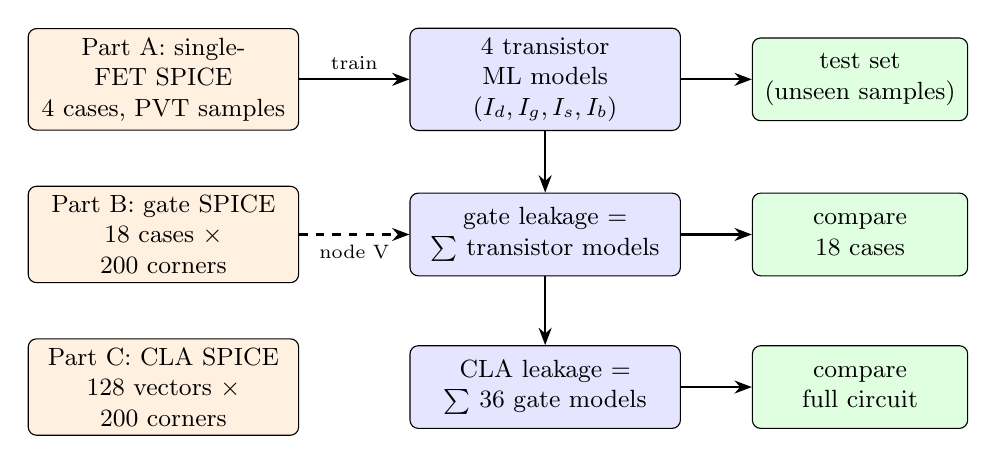
\begin{tikzpicture}[
  box/.style={draw, rounded corners=3pt, align=center, minimum height=1.05cm, text width=3.2cm, font=\small},
  spice/.style={box, fill=orange!12},
  ml/.style={box, fill=blue!10},
  cmp/.style={box, fill=green!12, text width=2.5cm},
  arr/.style={-{Stealth[length=2.2mm]}, thick}]
\node[spice] (s1) {Part A: single-FET SPICE\\ 4 cases, PVT samples};
\node[ml, right=1.4cm of s1] (m1) {4 transistor ML models\\ $(I_d, I_g, I_s, I_b)$};
\node[cmp, right=0.9cm of m1] (c1) {test set\\ (unseen samples)};
\node[spice, below=0.7cm of s1] (s2) {Part B: gate SPICE\\ 18 cases $\times$ 200 corners};
\node[ml, right=1.4cm of s2] (m2) {gate leakage =\\ $\sum$ transistor models};
\node[cmp, right=0.9cm of m2] (c2) {compare\\ 18 cases};
\node[spice, below=0.7cm of s2] (s3) {Part C: CLA SPICE\\ 128 vectors $\times$ 200 corners};
\node[ml, right=1.4cm of s3] (m3) {CLA leakage =\\ $\sum$ 36 gate models};
\node[cmp, right=0.9cm of m3] (c3) {compare\\ full circuit};
\draw[arr] (s1) -- node[above,font=\scriptsize]{train} (m1);
\draw[arr] (m1) -- (c1);
\draw[arr] (m1) -- (m2);
\draw[arr] (m2) -- (m3);
\draw[arr] (m2) -- (c2);
\draw[arr] (m3) -- (c3);
\draw[arr, dashed] (s2) -- node[below,font=\scriptsize]{node V} (m2);
\end{tikzpicture}
\caption{Hierarchical flow. Orange: SPICE; blue: ML; green: comparison against the SPICE result of the same
row. SPICE gate and circuit results are references only and are never used for training; the dashed ``node V''
arrow is the recorded internal node voltages that step 4 of the specification lets the gate ML use.}
\label{fig:flow}
\end{figure}

% ------------------------------------------------------------------------------------------
\section{Setup: technology, simulator and environment}
\begin{table}[H]
\centering
\caption{Technology and simulation setup.}
\begin{tabularx}{\textwidth}{lX}
\toprule
Model file & \code{models/45nm\_HP.pm} (PTM 45\,nm HP, BSIM4 level 54) \\
Nominal VDD & 1\,V (sampled 0.9--1.1\,V) \\
Channel length & $L = 45$\,nm \\
Widths & 45--360\,nm ($1$--$8\,L_\text{min}$) \\
Test circuit & 3-bit CLA adder, inputs $A$, $B$, $C_\text{in}$: all 128 combinations \\
Simulator & ngspice 44.2 (console build \code{ngspice\_con.exe}), batch mode \\
Software & Python 3.13, numpy 2.5.4, pandas 3.1.1, scikit-learn 1.9.1, LightGBM 4.7.0, PyTorch 2.8.0 (CPU) \\
\bottomrule
\end{tabularx}
\end{table}

Every netlist (transistor, gate, circuit) contains
\code{.options gmin=1e-18 abstol=1e-18 reltol=1e-6 vntol=1e-9}, and the single-transistor netlists drive every
terminal with its own voltage source (Fig.~\ref{fig:screen-netlist}). Results are read from ngspice ASCII raw
files (full double precision), not from printed logs. Currents are positive \emph{into} the device terminal,
$I = -i(V_\text{source})$. Process variation is written into a fresh model card for every sample: we found
that \code{altermod toxe} in ngspice 44.2 does not recompute the oxide-dependent BSIM4 terms (errors up to
$\approx 5\times$). Isolated non-converging circuits are retried with raised DC iteration limits (tolerances
unchanged).

\begin{figure}[H]
\centering
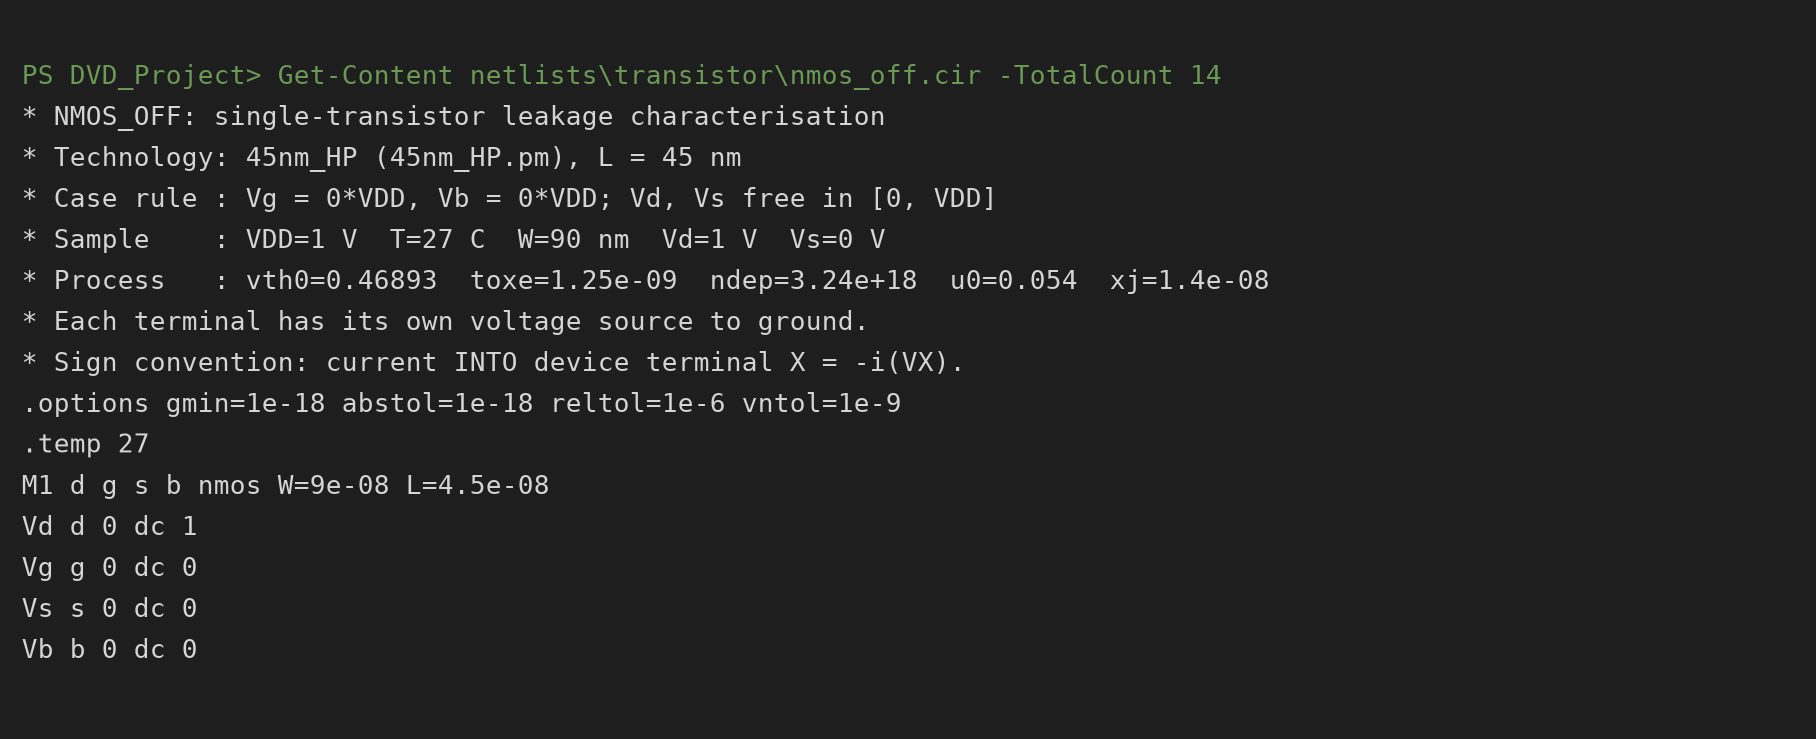
\includegraphics[width=0.92\textwidth]{screen_netlist.png}
\caption{Screenshot: header of the example single-transistor netlist (NMOS OFF). Each terminal has its own
source; the required \code{.options} line is present. The model card with the sample's process values follows
below these lines.}
\label{fig:screen-netlist}
\end{figure}

% ------------------------------------------------------------------------------------------
\section{Data generation}
\subsection{PVT sampling}
For each transistor sample, every parameter is drawn independently: VDD $\sim U(\pm 10\pct)$ is drawn first;
$V_d, V_s \sim U(0, \text{VDD})$; $W \sim U(1$--$8\,L_\text{min})$; $T \sim U(-40, 125)\,^\circ$C;
\code{vth0}, \code{toxe}, \code{ndep}, \code{u0}, \code{xj} $\sim U(\pm 10\pct)$ of the device's own nominal
value. $V_g$/$V_b$ follow the case: NMOS ON (VDD, 0), NMOS OFF (0, 0), PMOS ON (0, VDD), PMOS OFF (VDD, VDD).
Sample $k$ is drawn from \code{default\_rng([case\_seed, k // 1000])}, so every sample is reproducible on its
own. Seeds: data 1001 (+100 per case), split 2002, training 3003, gate/circuit corners 4004 (independent
evaluation corners 5005). A \emph{corner} draws VDD, $T$, one NMOS and one separate PMOS set of the five
process parameters, shared by all devices of that type.

\subsection{Datasets and split}
40{,}000 single-transistor simulations, 40{,}000 succeeded, 0 failed; regenerating from scratch reproduced the
four CSV files byte for byte. Each file has the columns \code{vdd, temp, w, vd, vs, vg, vb, vth0, toxe, ndep,
u0, xj, id, ig, is, ib} (Fig.~\ref{fig:screen-data}). Each case is split 70/15/15 (7{,}000 / 1{,}500 / 1{,}500)
with a fixed seed. Supplementary targeted samples (terminals near the rails, $|V_{ds}|$ down to 1\,nV) were
generated later for training only (4{,}000 + 4{,}000 per ON case, 2{,}000 + 2{,}000 per OFF case; separate files).

\begin{figure}[H]
\centering
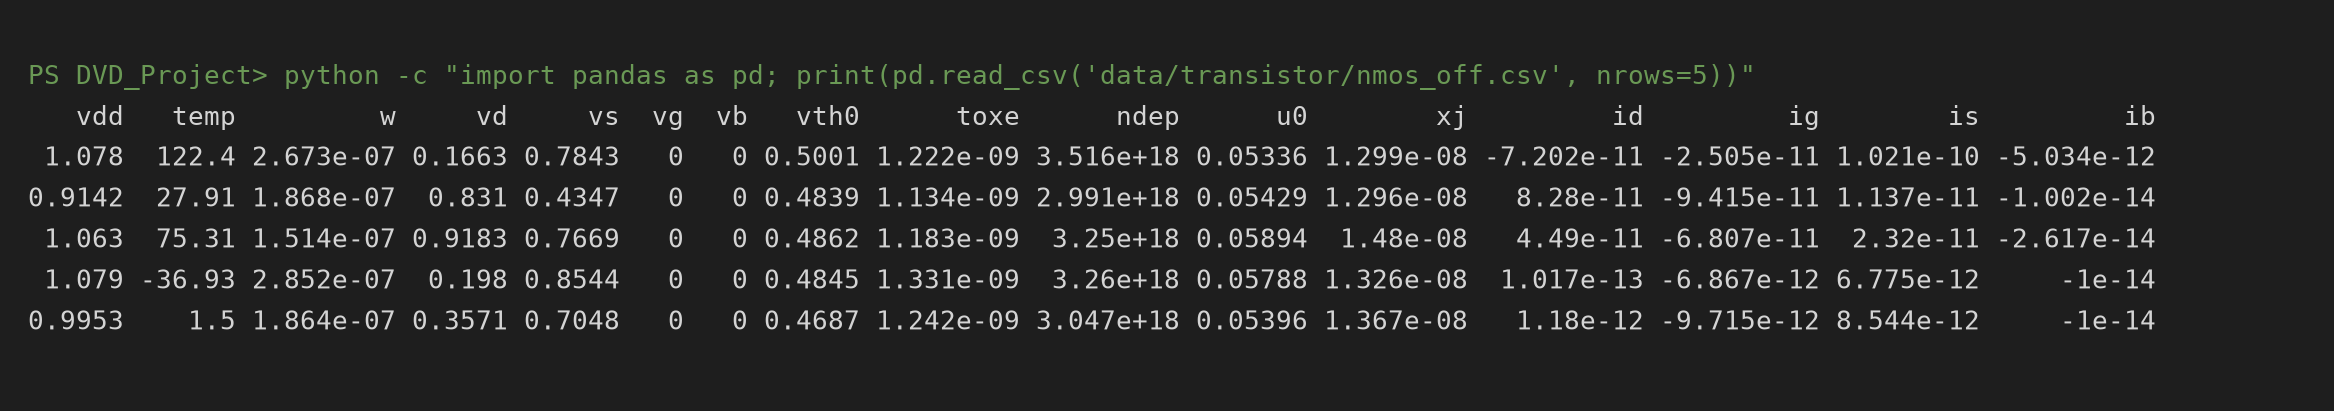
\includegraphics[width=\textwidth]{screen_dataset.png}
\caption{Screenshot: first rows of the NMOS OFF dataset (\code{data/transistor/nmos\_off.csv}).}
\label{fig:screen-data}
\end{figure}

\subsection{Data check}
\begin{table}[H]
\centering
\caption{Kirchhoff check: sum of the four terminal currents per sample.}
\begin{tabular}{lcccc}
\toprule
Case & max $|\Sigma I|$ (A) & median $|\Sigma I|$ (A) & p95 $|\Sigma I|$ (A) & over tolerance \\
\midrule
NMOS ON  & 1.90e-15 & 7.75e-17 & 3.55e-16 & 0 \\
NMOS OFF & 1.87e-23 & 4.19e-27 & 1.89e-25 & 0 \\
PMOS ON  & 1.86e-16 & 3.03e-17 & 8.78e-17 & 0 \\
PMOS OFF & 1.51e-15 & 8.82e-17 & 3.90e-16 & 0 \\
\bottomrule
\end{tabular}
\end{table}

The largest residuals ($\sim$1e-15\,A) occur only when all four currents are tiny; they do not depend on
gmin, reltol or vntol and are a fixed BSIM4 non-conservation. The physical trends were checked with the
other randomised inputs conditioned so they do not hide the effect ($|V_{ds}| \ge 0.5\,$VDD and the source
within 0.05\,VDD of its rail for OFF current). Partial-regression slopes from the dataset agree with
controlled SPICE sweeps:

\begin{table}[H]
\centering
\caption{Trend slopes: dataset (other inputs fixed) vs controlled SPICE sweep.}
\begin{tabular}{llccc}
\toprule
Trend & Device & Unit & Dataset & SPICE sweep \\
\midrule
OFF $|I_d|$ vs temperature & NMOS & decades / 10\,$^\circ$C & +0.112 & +0.093 \\
OFF $|I_d|$ vs $|$vth0$|$ & NMOS & decades / 10\,mV & $-0.115$ & $-0.113$ \\
ON $|I_g|$ vs toxe & NMOS & decades / 0.1\,nm & $-0.664$ & $-0.651$ \\
OFF $|I_d|$ vs temperature & PMOS & decades / 10\,$^\circ$C & +0.104 & +0.086 \\
OFF $|I_d|$ vs $|$vth0$|$ & PMOS & decades / 10\,mV & $-0.099$ & $-0.108$ \\
ON $|I_g|$ vs toxe & PMOS & decades / 0.1\,nm & $-0.588$ & $-0.585$ \\
\bottomrule
\end{tabular}
\end{table}

\begin{figure}[H]
\centering
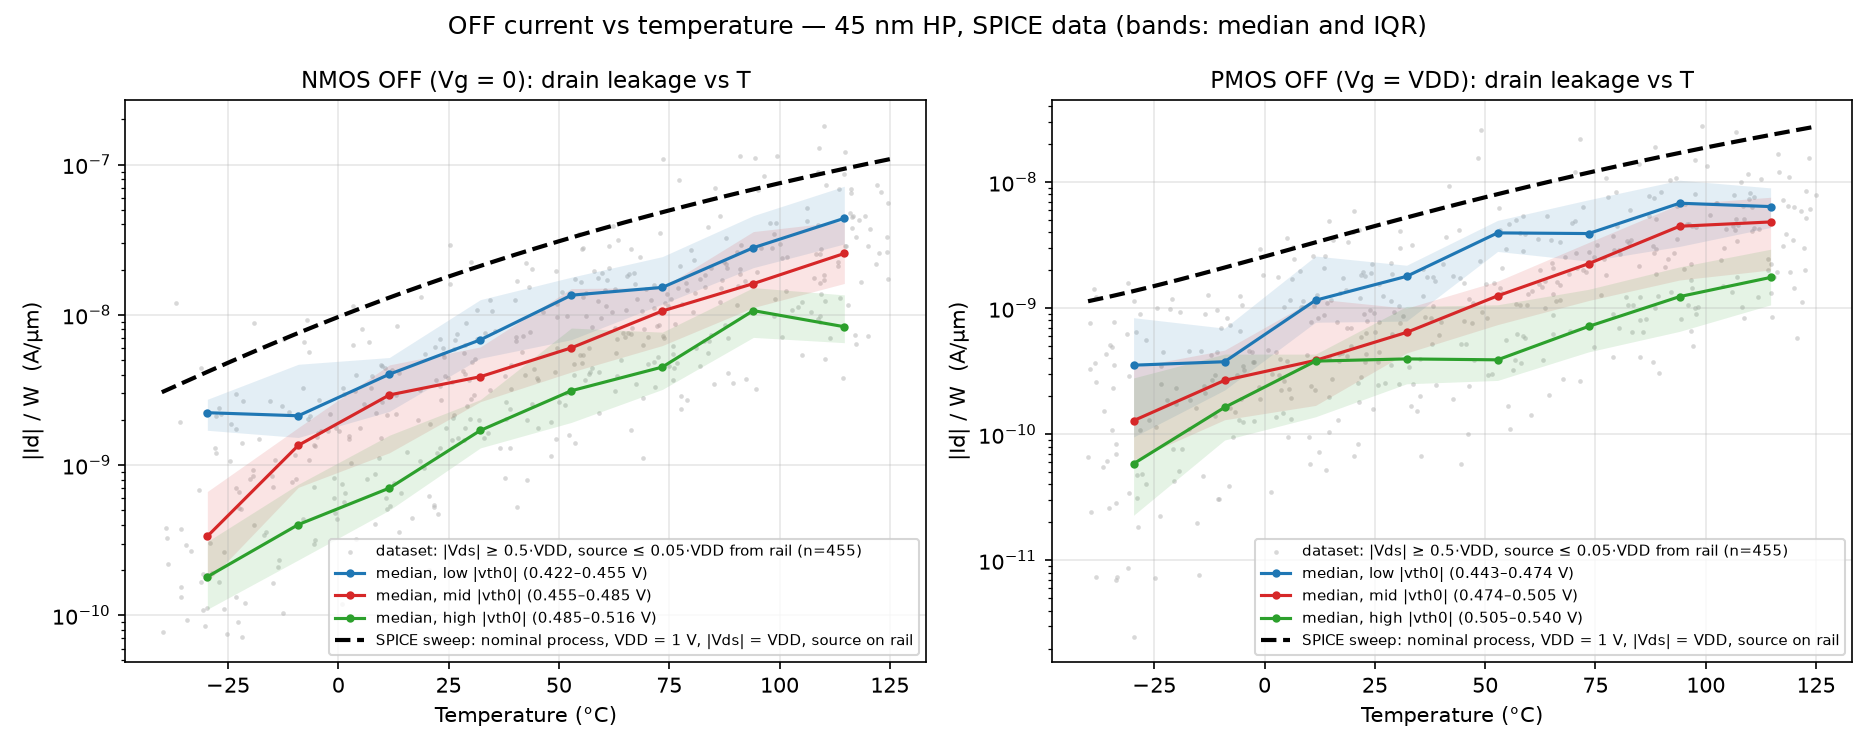
\includegraphics[width=0.8\textwidth]{fig1_fig_off_current_vs_temperature.png}
\caption{OFF current vs temperature (NMOS and PMOS).}
\end{figure}
\begin{figure}[H]
\centering
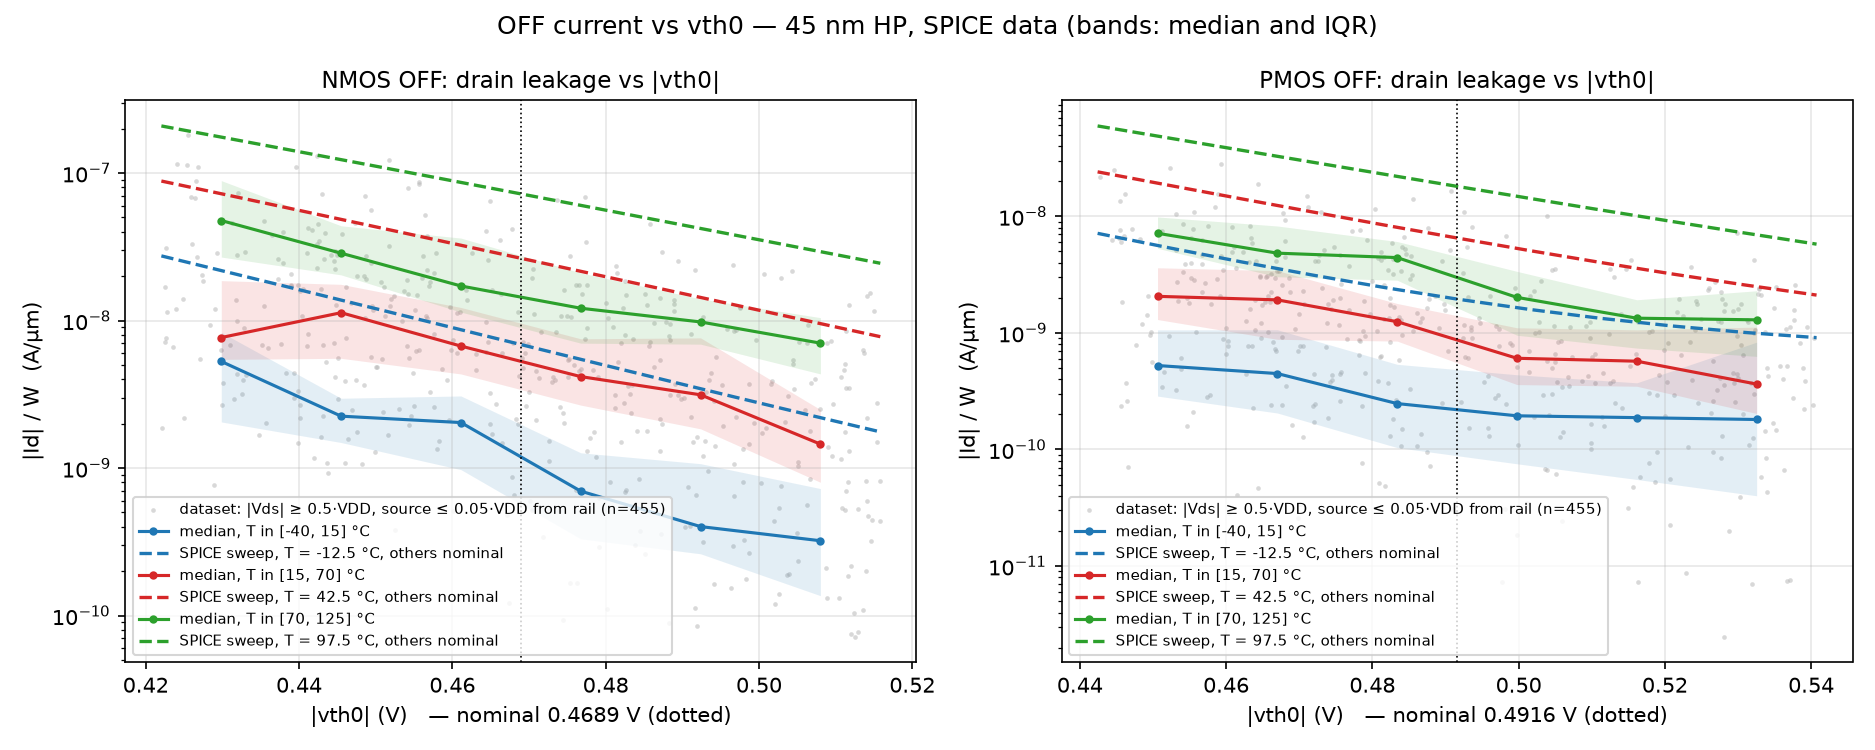
\includegraphics[width=0.8\textwidth]{fig2_fig_off_current_vs_vth0.png}
\caption{OFF current vs vth0.}
\end{figure}
\begin{figure}[H]
\centering
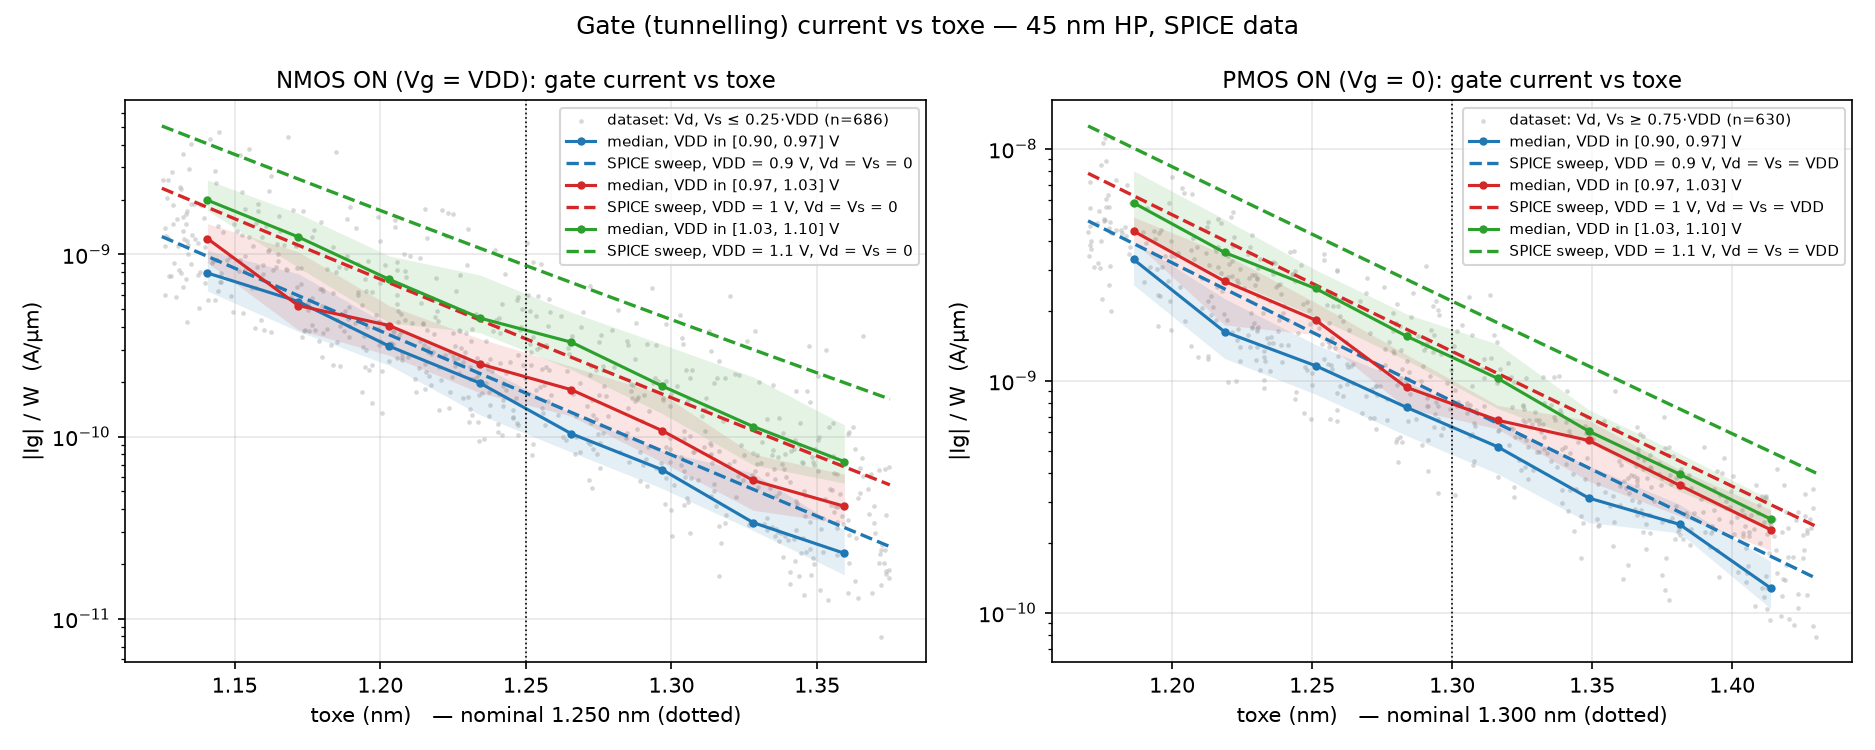
\includegraphics[width=0.8\textwidth]{fig3_fig_gate_current_vs_toxe.png}
\caption{Gate current vs toxe.}
\end{figure}

Other findings: OFF current falls about one decade per 0.1\,VDD of source offset (negative $V_{gs}$ plus body
effect, Fig.~\ref{fig:offset}); every non-nominal \code{toxe} triggers BSIM4's ``toxe $\neq$ toxp + dtox; dtox
ignored'' warning because the specification varies \code{toxe} only; the OFF-state body current is a nearly
constant $\sim$1e-14\,A drain-junction current (no junction area/perimeter in the netlists); and the OFF-state
$I_d$ flows against $V_{ds}$ in 28--36\pct\ of samples because the channel current and gate-to-drain
tunnelling nearly cancel.

\begin{figure}[H]
\centering
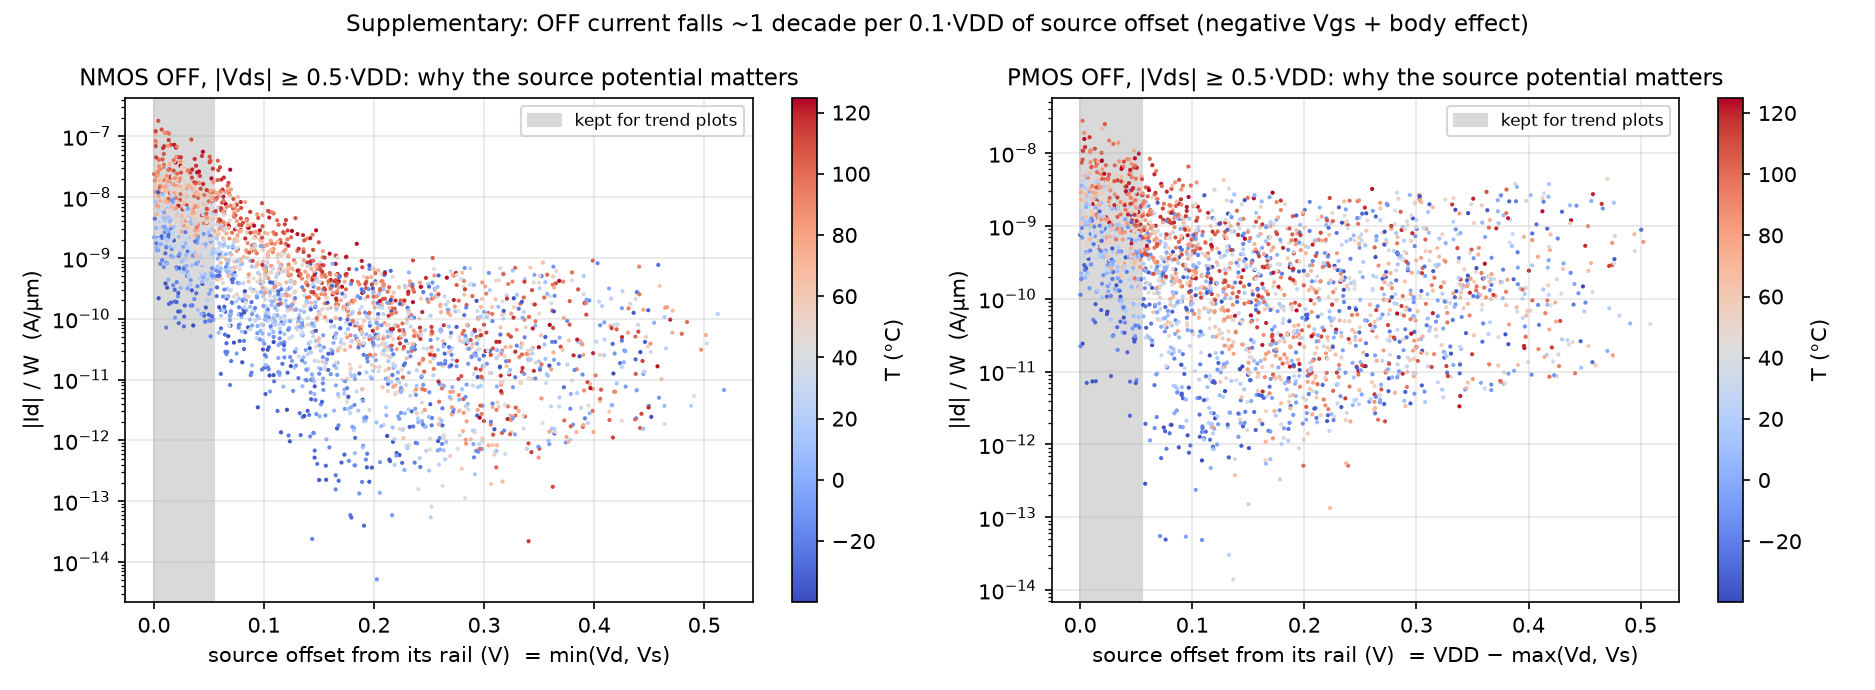
\includegraphics[width=0.8\textwidth]{fig4_fig_supp_off_current_vs_source_offset.png}
\caption{OFF current vs source offset from its rail: the reason the OFF-current trend plots are conditioned
on the source potential.}
\label{fig:offset}
\end{figure}

% ------------------------------------------------------------------------------------------
\section{Transistor models}
\subsection{Features, target and metric}
Features: VDD, $T$ (K), $\log_{10} W$, $V_d$, $V_s$, $V_{ds}$, $|V_{ds}|$, $V_{gs}$, $V_{gd}$, $V_{bs}$,
$V_{bd}$, source offset from its rail, the five process parameters relative to nominal, and (from v2 on)
$\operatorname{asinh}(V_{ds}/1\,\mu\text{V})$. Targets: all four currents jointly, transformed with
$\operatorname{asinh}(I/1\,\text{fA})$, a signed logarithm that is smooth through zero. Scalers are fit on the
training data; tuning and selection use the validation set only. Error metric:
\[
e = \frac{|I_\text{pred} - I_\text{SPICE}|}{\max(|I_\text{SPICE}|, 1\,\text{fA})},\qquad
\text{mean accuracy} = 100\pct \cdot \bigl(1 - \overline{e}\bigr).
\]

\begin{table}[H]
\centering
\caption{Target-transform study (LightGBM, validation median relative error).}
\begin{tabular}{lccccc}
\toprule
Transform & NMOS OFF & NMOS ON & PMOS OFF & PMOS ON & Mean \\
\midrule
sign + $\log_{10}|I|$ & 6.89\pct & 8.11\pct & 5.52\pct & 8.49\pct & 7.25\pct \\
$\operatorname{asinh}(I/10^{-15})$ & 7.82\pct & 8.68\pct & 5.48\pct & 8.78\pct & 7.69\pct \\
$\operatorname{asinh}(I/10^{-18})$ & 8.98\pct & 9.39\pct & 5.92\pct & 9.30\pct & 8.40\pct \\
$\operatorname{asinh}(I/10^{-12})$ & 9.57\pct & 10.93\pct & 7.43\pct & 11.52\pct & 9.86\pct \\
$\operatorname{asinh}(I/10^{-9})$ & 21.73\pct & 27.98\pct & 13.46\pct & 29.31\pct & 23.12\pct \\
linear & 33.26\pct & 34.71\pct & 15.10\pct & 33.79\pct & 29.21\pct \\
\bottomrule
\end{tabular}
\end{table}
Sign + $\log_{10}|I|$ scored slightly better but needs a separate sign classifier per terminal;
$\operatorname{asinh}(I/1\,\text{fA})$ is the best transform that every algorithm can use in a single
regression model.

\subsection{Model comparison (4 model types $\times$ 4 cases)}
\begin{table}[H]
\centering
\caption{Validation results, best configuration of each model type (mean over the four terminals).}
\begin{tabular}{llccc}
\toprule
Case & Model & $R^2$ (asinh space) & Median rel.\ error & p95 rel.\ error \\
\midrule
NMOS OFF & MLP & 0.9973 & 1.55\pct & 9.42\pct \\
 & LightGBM & 0.9906 & 7.15\pct & 55.26\pct \\
 & Random forest & 0.9685 & 21.99\pct & 122.40\pct \\
 & Polynomial ridge & 0.9416 & 46.60\pct & 318.98\pct \\
\midrule
NMOS ON & MLP & 0.9982 & 2.25\pct & 12.62\pct \\
 & LightGBM & 0.9971 & 7.94\pct & 42.67\pct \\
 & Random forest & 0.9876 & 25.10\pct & 186.25\pct \\
 & Polynomial ridge & 0.9606 & 56.83\pct & 8127.03\pct \\
\midrule
PMOS OFF & MLP & 0.9988 & 1.15\pct & 7.02\pct \\
 & LightGBM & 0.9817 & 5.04\pct & 54.98\pct \\
 & Random forest & 0.9551 & 18.07\pct & 85.03\pct \\
 & Polynomial ridge & 0.9367 & 38.39\pct & 272.38\pct \\
\midrule
PMOS ON & MLP & 0.9973 & 2.57\pct & 16.52\pct \\
 & LightGBM & 0.9976 & 7.93\pct & 44.07\pct \\
 & Random forest & 0.9873 & 26.04\pct & 195.66\pct \\
 & Polynomial ridge & 0.9614 & 56.43\pct & 5289.52\pct \\
\bottomrule
\end{tabular}
\end{table}

Main hyperparameters (best configuration per case, chosen on validation from a grid):
\begin{itemize}[nosep]
\item \textbf{MLP}: 3 hidden layers of 128, tanh, L-BFGS, $\alpha = 10^{-5}$;
\item \textbf{LightGBM}: 4000 trees, learning rate 0.03, 63 leaves;
\item \textbf{Random forest}: 300 trees, all features per split, minimum leaf size 1;
\item \textbf{Polynomial ridge}: degree 3, $\alpha = 0.01$.
\end{itemize}
The MLP won every case by 3--5$\times$: the currents are smooth exponential functions of the inputs, which a
smooth network represents well, while trees give piecewise-constant fits over 11 decades and polynomial ridge
cannot follow the exponentials.

\subsection{Model history and final choice}
v1 used scikit-learn's L-BFGS MLP. v2 added the signed-log $V_{ds}$ feature and the targeted samples, which
fixed the ON-state $I_d/I_s$ near $V_{ds} = 0$ (the regime of ON transistors inside static gates; the switch of
the OFF models to v2 is a disclosed amendment). An improvement phase then found that every earlier fit had
stopped at scikit-learn's 3{,}000-iteration cap with training error $\approx$ validation error, i.e.\ the
networks were under-fitted. The same network trained with PyTorch full-batch L-BFGS for 15--20k iterations (E2),
plus extra targeted data where a train/validation gap appeared (E5), and ensembles (E1, E6), were compared with a
validation score fixed in advance (mean over the original and targeted validation sets of median + 0.1$\cdot$p95):

\begin{table}[H]
\centering
\caption{Improvement experiments: validation score (lower is better).}
\begin{tabular}{lcccc}
\toprule
Experiment & NMOS OFF & NMOS ON & PMOS OFF & PMOS ON \\
\midrule
E0 baseline (v2) & 0.0442 & 0.1184 & 0.0459 & 0.1003 \\
E1 ensemble of v2 fits & 0.0384 & 0.0914 & 0.0396 & 0.0834 \\
E2 PyTorch L-BFGS, same data & 0.0173 & 0.0655 & 0.0209 & 0.0500 \\
E5 PyTorch + extra targeted data & \textbf{0.0120} & 0.0442 & \textbf{0.0138} & \textbf{0.0294} \\
E6 ensemble of E2 and E5 & 0.0121 & \textbf{0.0380} & 0.0157 & 0.0341 \\
\bottomrule
\end{tabular}
\end{table}
Final models: NMOS ON = E6 (ensemble), NMOS OFF, PMOS ON and PMOS OFF = E5.

\begin{figure}[H]
\centering
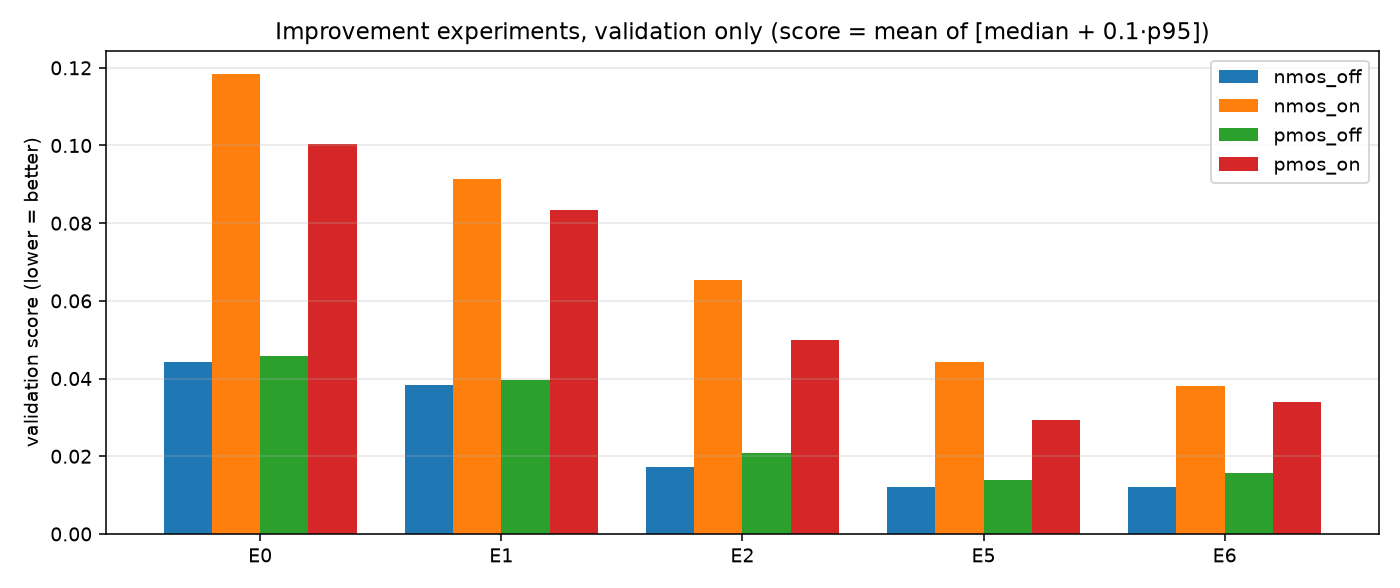
\includegraphics[width=0.85\textwidth]{fig10_validation_experiments.png}
\caption{Validation score of the improvement experiments.}
\end{figure}

\subsection{Test results of the chosen models}
\begin{table}[H]
\centering
\caption{Final models on the independent test set (1{,}500 fresh samples per case, specification distribution).}
\begin{tabular}{lcccccccc}
\toprule
 & \multicolumn{4}{c}{Median rel.\ error per terminal} & \multicolumn{4}{c}{Mean over the four terminals} \\
\cmidrule(lr){2-5}\cmidrule(lr){6-9}
Case & $I_d$ & $I_g$ & $I_s$ & $I_b$ & Median & p95 & $R^2$ (asinh) & Sign acc. \\
\midrule
NMOS ON  & 0.94\pct & 0.29\pct & 0.93\pct & 0.35\pct & 0.63\pct & 3.10\pct & 0.999991 & 100.0\pct \\
NMOS OFF & 0.77\pct & 0.30\pct & 0.89\pct & 0.16\pct & 0.53\pct & 3.30\pct & 0.999653 & 100.0\pct \\
PMOS ON  & 1.16\pct & 0.33\pct & 1.13\pct & 0.47\pct & 0.77\pct & 3.75\pct & 0.999979 & 100.0\pct \\
PMOS OFF & 0.67\pct & 0.31\pct & 0.67\pct & 0.38\pct & 0.51\pct & 3.40\pct & 0.997653 & 99.9\pct \\
\bottomrule
\end{tabular}
\end{table}
Mean over cases and terminals: median
0.61\pct, p95 3.39\pct, mean accuracy \textbf{98.56\pct}. On the near-rail / small-$|V_{ds}|$ test set: median
1.07\pct, p95 29.02\pct (a mean-based accuracy is not meaningful there because the currents cross zero).

\begin{figure}[H]
\centering
\begin{subfigure}{0.49\textwidth}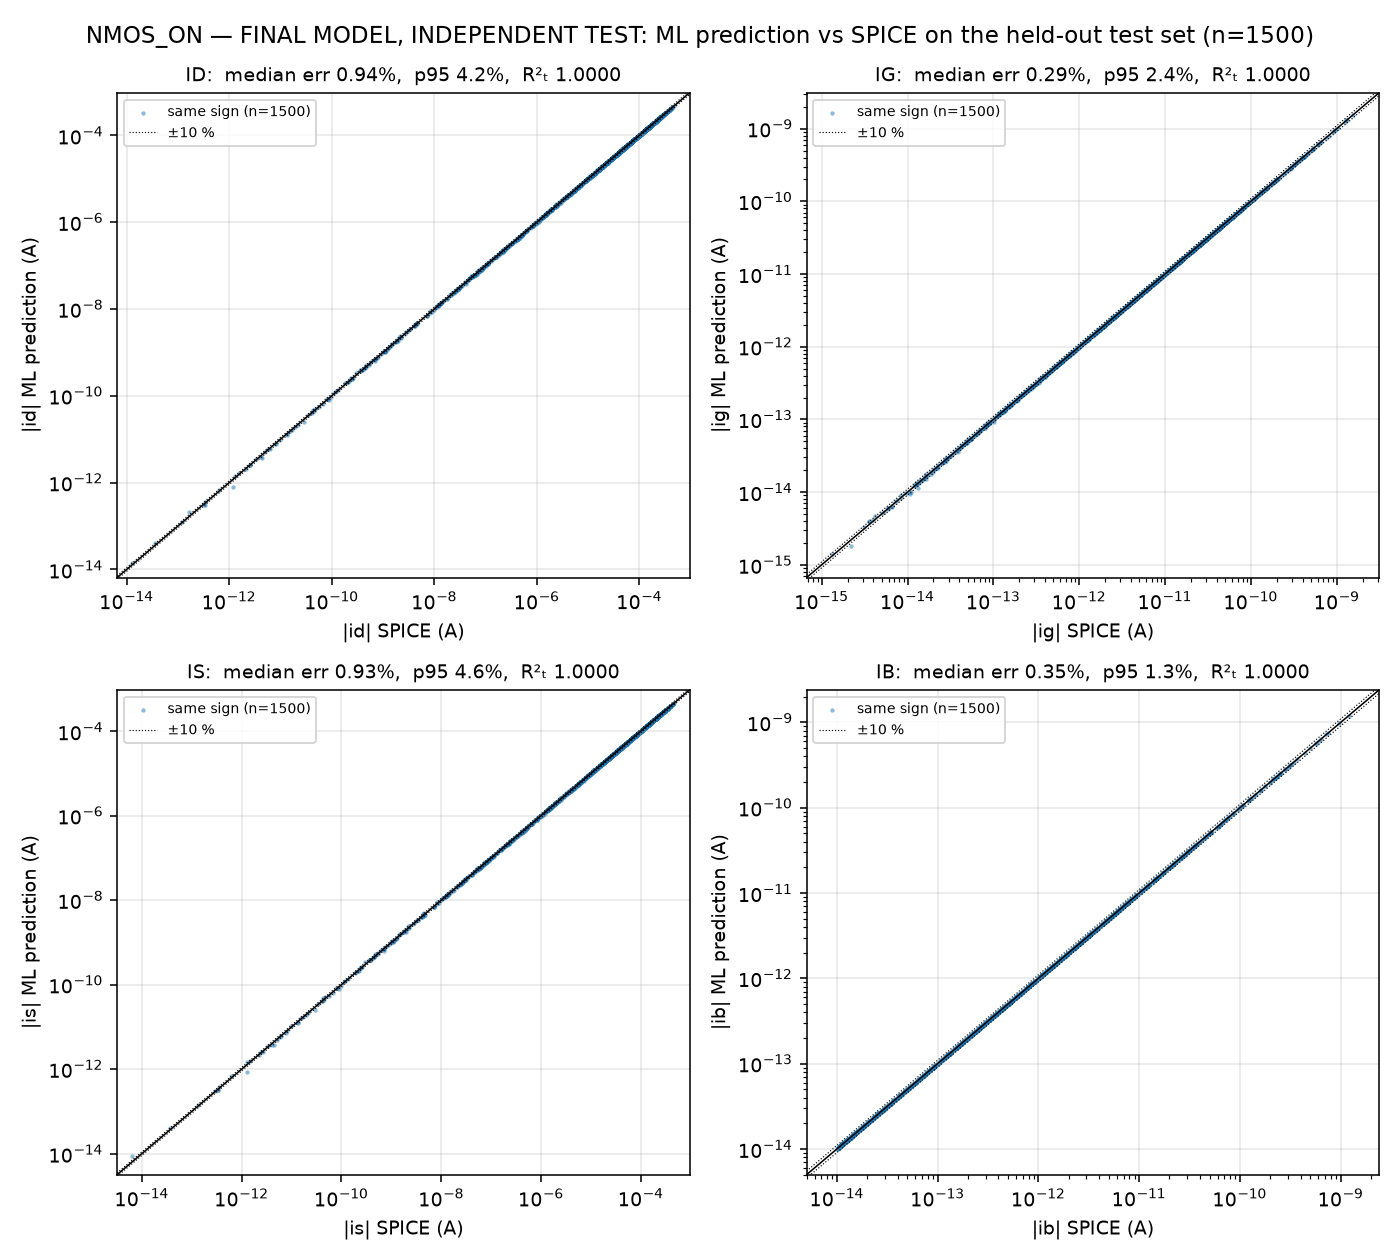
\includegraphics[width=\textwidth]{fig5_nmos_on.png}\caption{NMOS ON}\end{subfigure}
\begin{subfigure}{0.49\textwidth}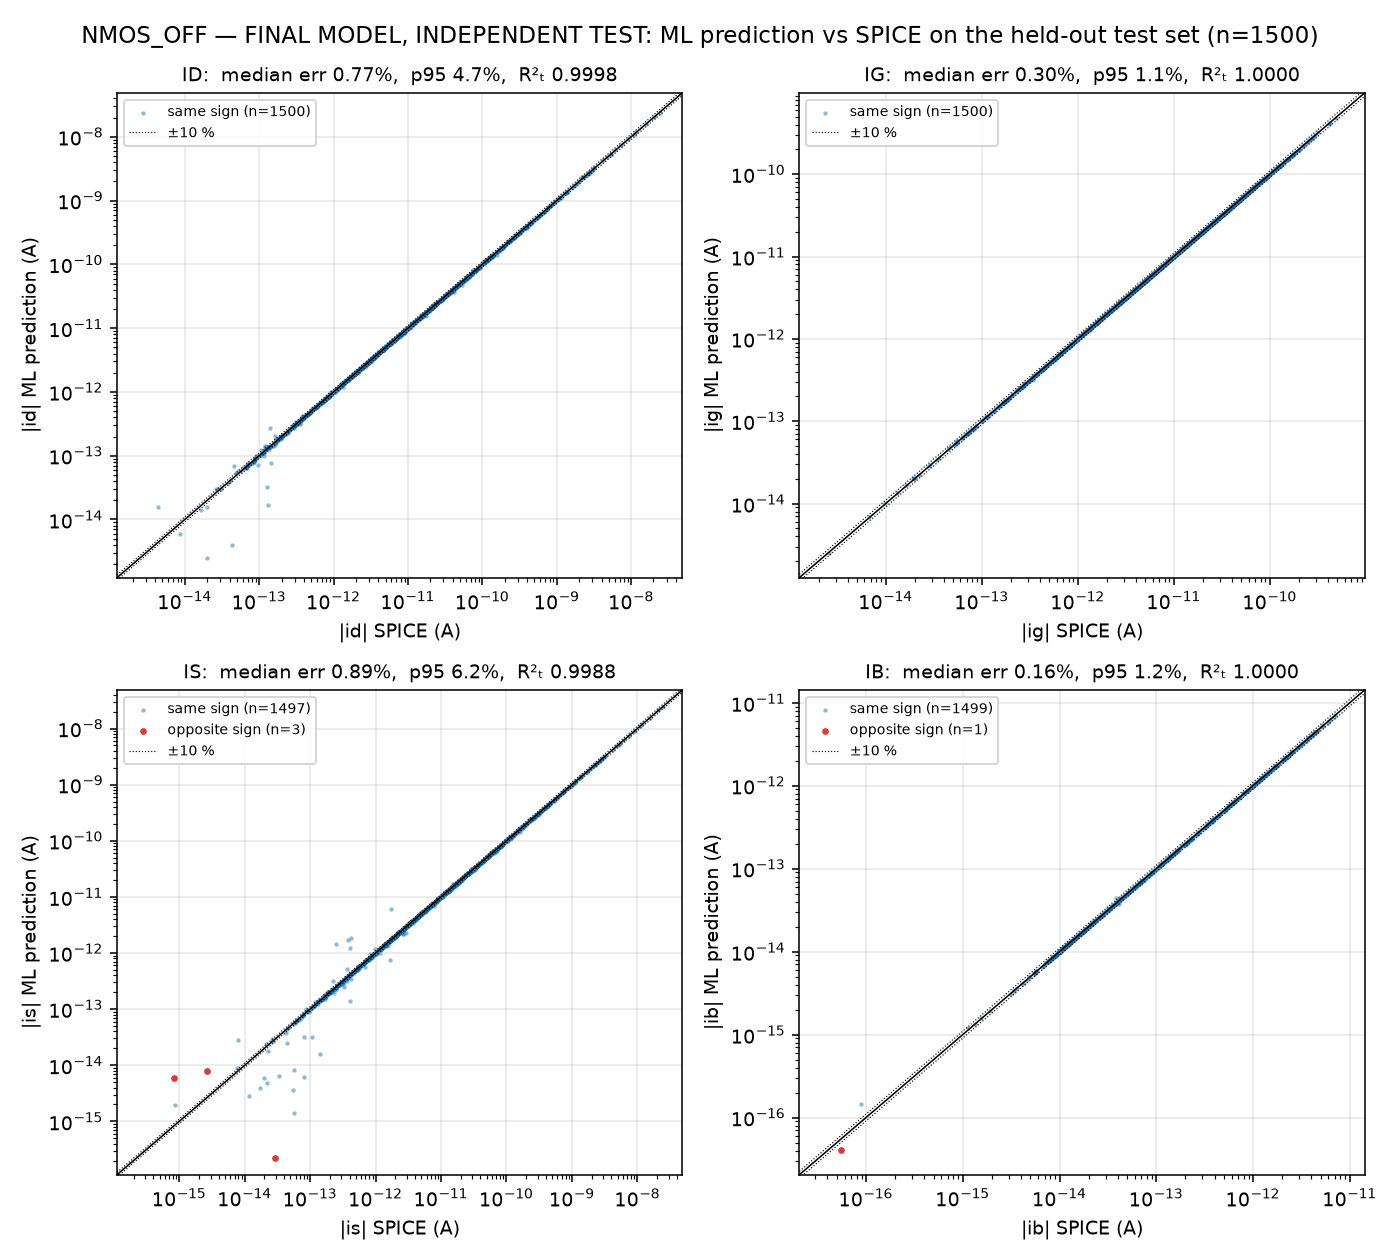
\includegraphics[width=\textwidth]{fig5_nmos_off.png}\caption{NMOS OFF}\end{subfigure}\\[4pt]
\begin{subfigure}{0.49\textwidth}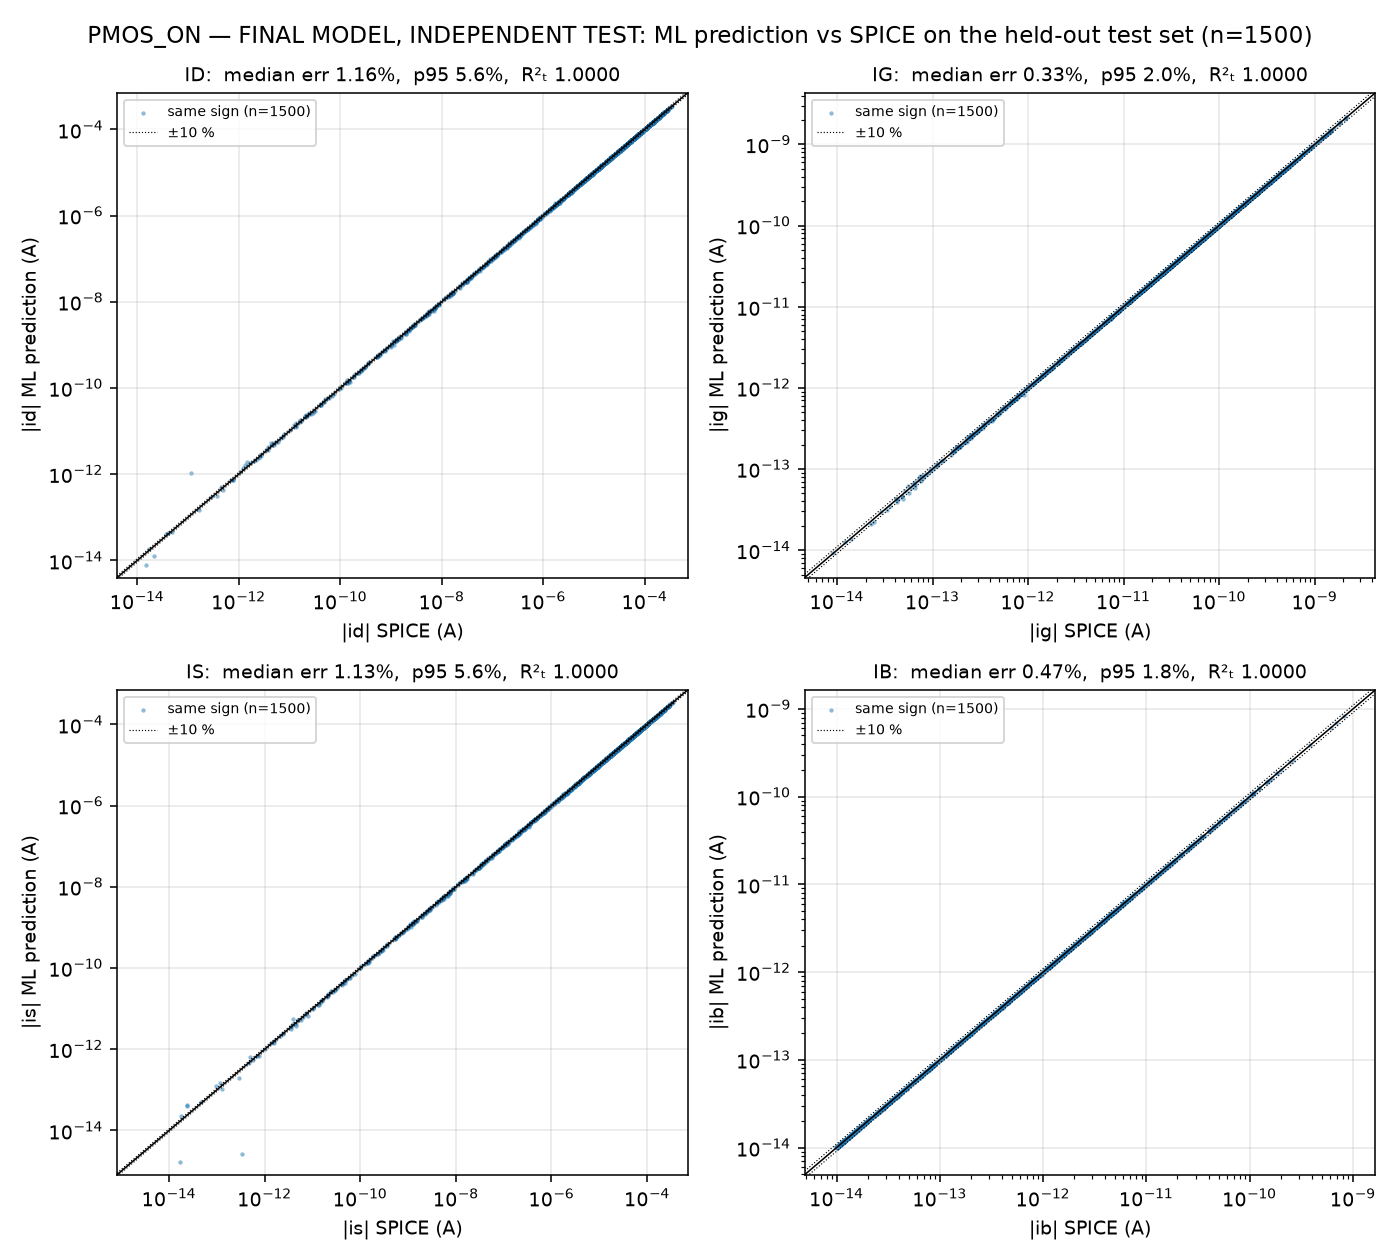
\includegraphics[width=\textwidth]{fig5_pmos_on.png}\caption{PMOS ON}\end{subfigure}
\begin{subfigure}{0.49\textwidth}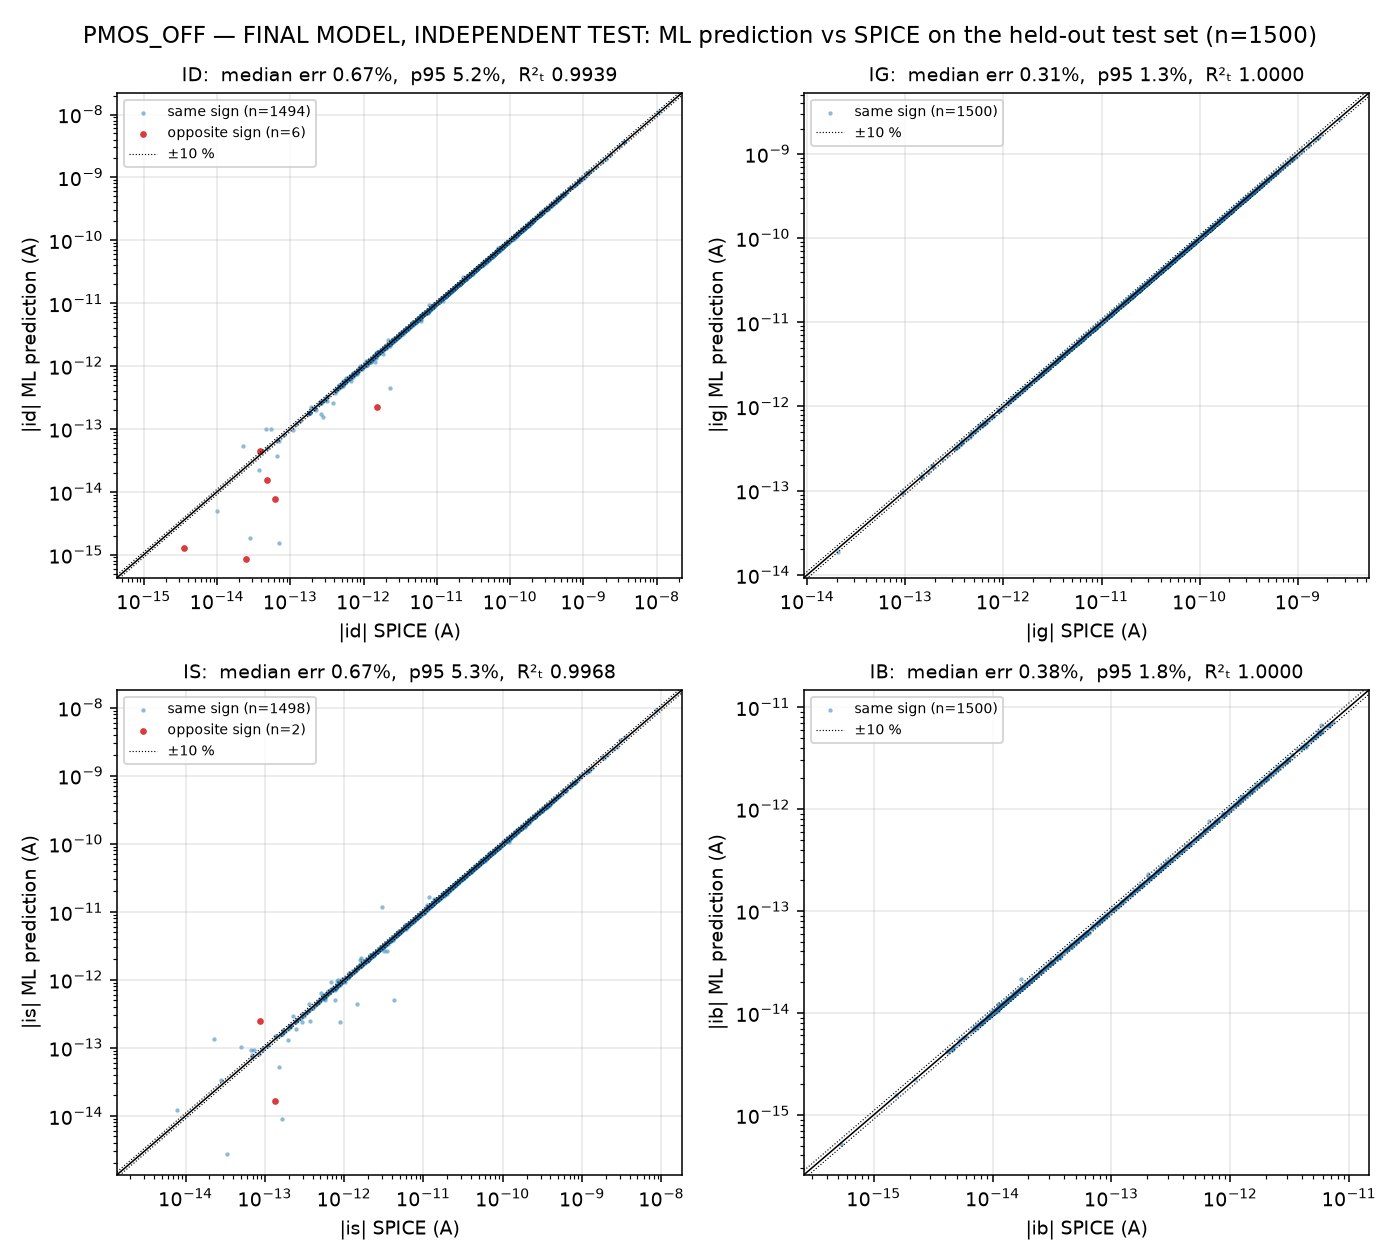
\includegraphics[width=\textwidth]{fig5_pmos_off.png}\caption{PMOS OFF}\end{subfigure}
\caption{Predicted vs SPICE terminal currents for each case (final models, independent test set).}
\end{figure}

% ------------------------------------------------------------------------------------------
\section{Gate-level validation}
\subsection{Gates and sizing}
Standard static CMOS gates; AND2 and OR2 are a NAND2 or NOR2 followed by an inverter and are simulated as one
complete netlist (Fig.~\ref{fig:gates}). Sizing is not given in the specification; equal-drive sizing is used:
unit inverter $W_n = 2L_\text{min}$ (90\,nm), $W_p = 4L_\text{min}$ (180\,nm), series pairs $2\times$ (NAND2 NMOS
180\,nm, NOR2 PMOS 360\,nm). All widths lie inside the ML training range. NMOS bodies are tied to 0, PMOS
bodies to VDD.

\begin{figure}[H]
\centering
\begin{circuitikz}[font=\small]
% ---------------- INV
\begin{scope}[shift={(0,0)}]
\node[pmos, anchor=S] (p) at (0,5) {};
\draw (p.S) -- ++(0,0.3) node[above]{VDD};
\coordinate (o) at ($(p.D)+(0,-0.4)$);
\draw (p.D) -- (o);
\node[nmos, anchor=D] (n) at (o) {};
\draw (n.S) node[ground]{};
\draw (p.G) -- ++(-0.45,0) coordinate (g1);
\draw (n.G) -- ++(-0.45,0) coordinate (g2);
\draw (g1) -- (g2);
\draw ($(g1)!0.5!(g2)$) to[short,*-o] ++(-0.6,0) node[left]{$A$};
\draw (o) to[short,*-o] ++(1.0,0) node[right]{out};
\node at (0,-1.6) {INV};
\end{scope}
% ---------------- NAND2
\begin{scope}[shift={(4.6,0)}]
\node[pmos, anchor=S] (pa) at (-0.9,5) {};
\node[pmos, anchor=S] (pb) at (0.9,5) {};
\draw (pa.S) -- (pb.S);
\draw (0,5) -- ++(0,0.3) node[above]{VDD};
\coordinate (o) at ($(pa.D)!0.5!(pb.D)+(0,-0.4)$);
\draw (pa.D) |- (o) -| (pb.D);
\node[nmos, anchor=D] (na) at (o) {};
\node[nmos, anchor=D] (nb) at (na.S) {};
\draw (na.S) node[circ]{} node[right=3pt]{$x$};
\draw (nb.S) node[ground]{};
\draw (pa.G) node[left]{$A$};
\draw (pb.G) node[left]{$B$};
\draw (na.G) node[left]{$A$};
\draw (nb.G) node[left]{$B$};
\draw (o) to[short,*-o] ++(1.6,0) node[right]{out};
\node at (0,-1.6) {NAND2};
\end{scope}
% ---------------- NOR2
\begin{scope}[shift={(9.6,0)}]
\node[pmos, anchor=S] (pa) at (0,6.2) {};
\draw (pa.S) -- ++(0,0.3) node[above]{VDD};
\node[pmos, anchor=S] (pb) at (pa.D) {};
\draw (pa.D) node[circ]{} node[right=3pt]{$y$};
\coordinate (o) at ($(pb.D)+(0,-0.4)$);
\draw (pb.D) -- (o);
\draw ($(o)+(-0.9,0)$) -- ($(o)+(0.9,0)$);
\node[nmos, anchor=D] (na) at ($(o)+(-0.9,0)$) {};
\node[nmos, anchor=D] (nb) at ($(o)+(0.9,0)$) {};
\draw (na.S) -- (nb.S);
\draw ($(na.S)!0.5!(nb.S)$) node[ground]{};
\draw (pa.G) node[left]{$A$};
\draw (pb.G) node[left]{$B$};
\draw (na.G) node[left]{$A$};
\draw (nb.G) node[left]{$B$};
\draw ($(o)+(0.9,0)$) to[short,-o] ++(0.9,0) node[right]{out};
\draw (o) node[circ]{};
\node at (0,-1.6) {NOR2};
\end{scope}
\end{circuitikz}
\caption{Gate schematics with the internal nodes of the specification: $x$ between the series NMOS of NAND2 and
$y$ between the series PMOS of NOR2. AND2/OR2 add an inverter on the NAND2/NOR2 output (node $n_1$).}
\label{fig:gates}
\end{figure}

\subsection{SPICE reference}
200 corners $\times$ 18 cases = 3{,}600 SPICE runs (0 failed, 0 logic errors). Gate inputs are applied at exactly
0 or VDD. Leakage is the static power divided by VDD,
\[
I_\text{leak} = \frac{1}{\text{VDD}} \sum_k V_k\,\bigl(-i(V_k)\bigr)
\]
over the VDD rail and the input sources (so gate tunnelling drawn from inputs held high is included). Every
transistor terminal has a 0\,V current probe; $\sum V I$ over all terminals equals the source power to 1e-6.
Fig.~\ref{fig:screen-ngspice} shows the example NAND2 netlist being simulated.

\begin{figure}[H]
\centering
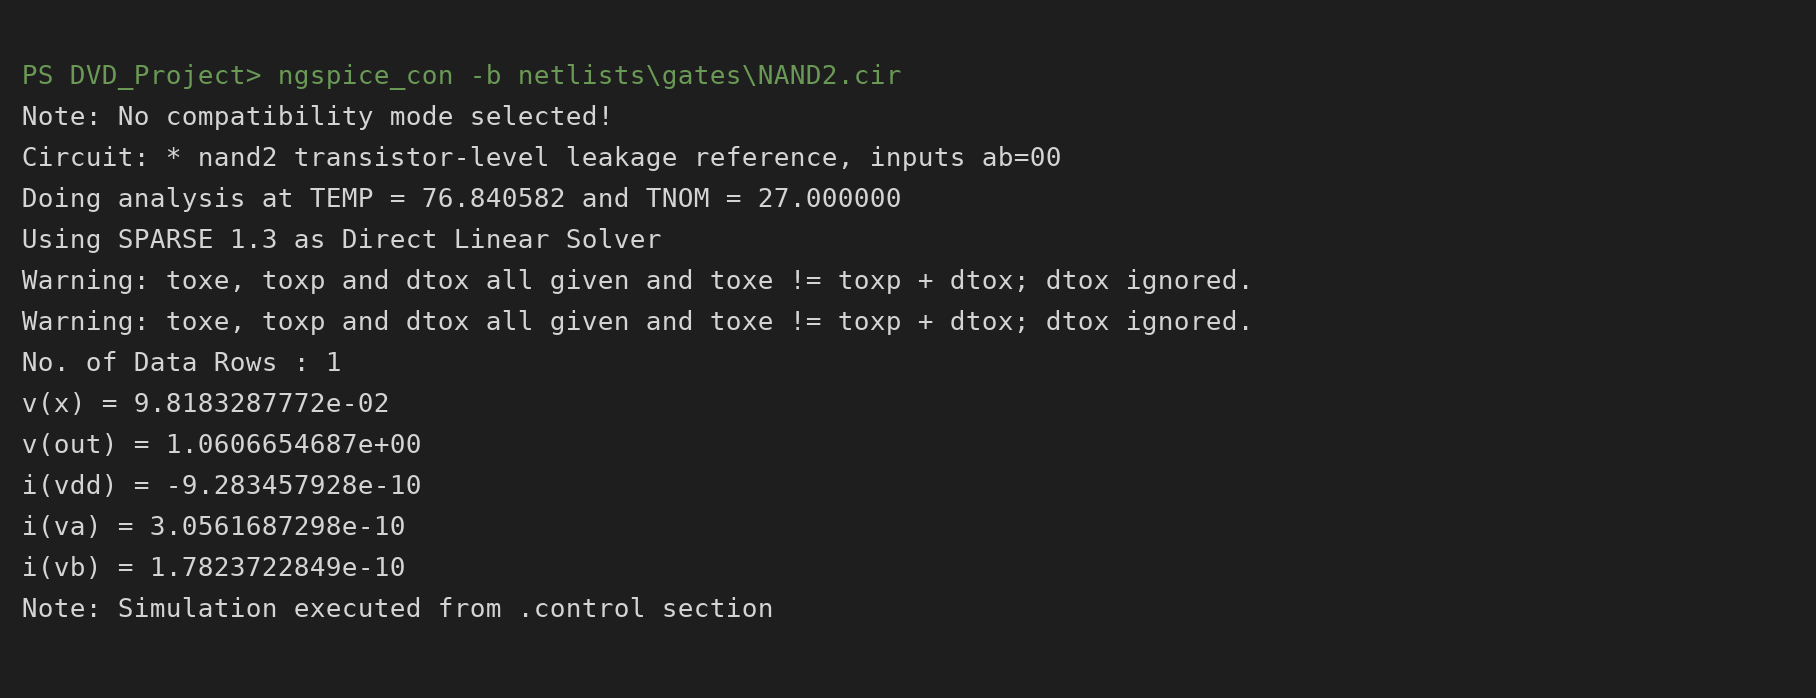
\includegraphics[width=0.85\textwidth]{screen_ngspice.png}
\caption{Screenshot: ngspice running the example NAND2 netlist (input 00, corner 0). The two warnings are the
expected BSIM4 \code{toxe} note discussed in the data check.}
\label{fig:screen-ngspice}
\end{figure}

\subsection{ML prediction}
For the same gates, inputs and corners, each transistor's $V_d, V_g, V_s, V_b$ follow from its connections:
inputs exactly 0/VDD, bodies on the rails, and the internal and output node voltages ($out$, $x$, $y$, $n_1$)
taken from the SPICE runs, as step 4 of the specification prescribes. The ON/OFF model is chosen from the gate
bias. Gate leakage is computed from the predicted currents as
\[
I_\text{leak} = \frac{1}{\text{VDD}} \sum_\text{transistors}
\bigl[(V_d - V_s) I_d + (V_g - V_s) I_g + (V_b - V_s) I_b\bigr],
\]
which equals the SPICE definition by Tellegen's theorem, is KCL-consistent per device and is insensitive to
the large ON-channel currents at $V_{ds} \approx 0$. Fed with SPICE's own transistor currents this formula
reproduces the SPICE leakage of all 3{,}600 cases. Inference runs with subprocess execution blocked, so no
hidden SPICE call is possible.

For every gate record the result files list the SPICE leakage, the ML leakage, the SPICE-measured node
voltages (columns \code{spice\_node\_*}) and, next to them, the node voltages supplied to the transistor
models (columns \code{ml\_input\_node\_*}). The ML-input voltages are the SPICE reference voltages used as
model inputs; they are not predicted by ML. They are read back from the actual model inputs and checked to be
identical for every record (Fig.~\ref{fig:screen-nodes}).

\begin{figure}[H]
\centering
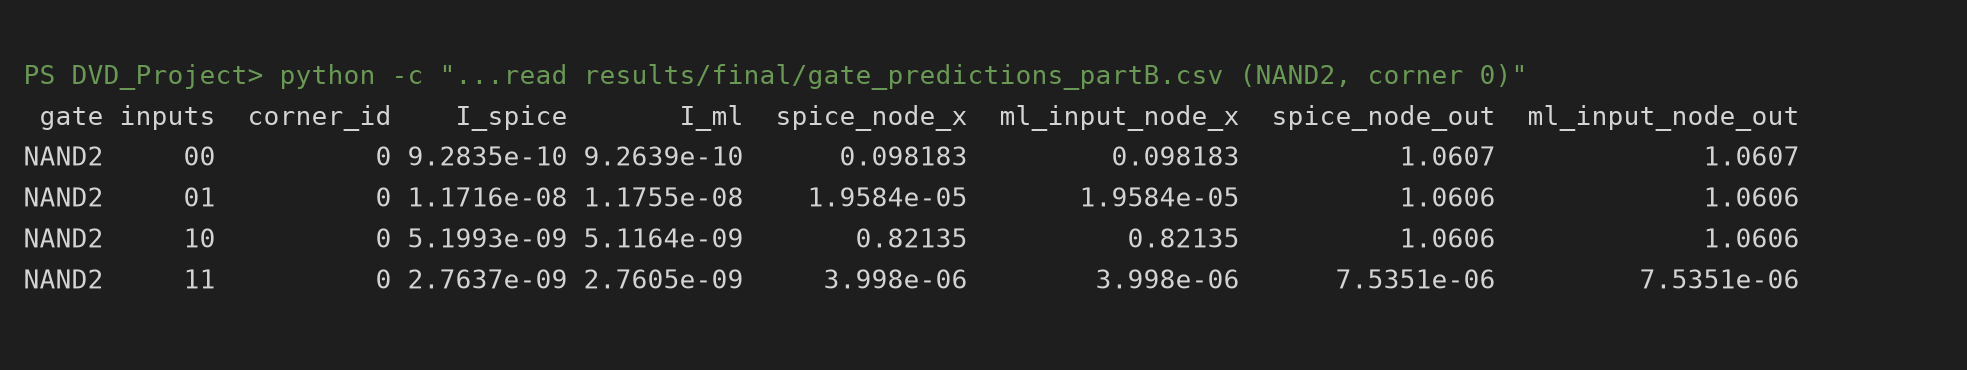
\includegraphics[width=\textwidth]{screen_nodes.png}
\caption{Screenshot: gate result file for NAND2 at corner 0, with SPICE and ML leakage and the SPICE node
voltages next to the voltages given to the transistor models.}
\label{fig:screen-nodes}
\end{figure}

\subsection{Gate results}
\begin{table}[H]
\centering
\caption{All 18 gate/input cases, final models, 200 Part B corners each.}
\begin{tabular}{llccccc}
\toprule
Gate & Inputs & SPICE median (A) & ML median (A) & Bias & Median err & p95 err \\
\midrule
INV & 0 & 2.564e-09 & 2.539e-09 & $-0.19$\pct & 0.77\pct & 2.48\pct \\
INV & 1 & 1.418e-09 & 1.420e-09 & $+0.11$\pct & 0.77\pct & 2.86\pct \\
NAND2 & 00 & 1.050e-09 & 1.043e-09 & $+0.05$\pct & 0.55\pct & 2.03\pct \\
NAND2 & 01 & 5.126e-09 & 5.118e-09 & $+0.17$\pct & 0.76\pct & 2.40\pct \\
NAND2 & 10 & 2.352e-09 & 2.356e-09 & $-0.23$\pct & 0.84\pct & 2.52\pct \\
NAND2 & 11 & 3.046e-09 & 3.020e-09 & $+0.06$\pct & 0.74\pct & 2.72\pct \\
NOR2 & 00 & 6.452e-09 & 6.425e-09 & $-0.23$\pct & 0.77\pct & 2.36\pct \\
NOR2 & 01 & 3.572e-09 & 3.599e-09 & $-0.13$\pct & 0.85\pct & 4.26\pct \\
NOR2 & 10 & 9.973e-10 & 9.793e-10 & $-0.87$\pct & 1.29\pct & 4.06\pct \\
NOR2 & 11 & 5.151e-10 & 5.253e-10 & $+0.76$\pct & 1.57\pct & 5.53\pct \\
AND2 & 00 & 2.627e-09 & 2.631e-09 & $+0.04$\pct & 0.50\pct & 2.29\pct \\
AND2 & 01 & 7.476e-09 & 7.463e-09 & $+0.12$\pct & 0.66\pct & 1.94\pct \\
AND2 & 10 & 4.569e-09 & 4.553e-09 & $-0.11$\pct & 0.61\pct & 2.00\pct \\
AND2 & 11 & 6.618e-09 & 6.631e-09 & $-0.09$\pct & 0.64\pct & 2.21\pct \\
OR2 & 00 & 8.622e-09 & 8.584e-09 & $-0.16$\pct & 0.68\pct & 2.09\pct \\
OR2 & 01 & 7.574e-09 & 7.519e-09 & $-0.17$\pct & 0.77\pct & 2.62\pct \\
OR2 & 10 & 4.280e-09 & 4.220e-09 & $-0.37$\pct & 0.76\pct & 2.39\pct \\
OR2 & 11 & 3.382e-09 & 3.411e-09 & $-0.01$\pct & 0.77\pct & 2.57\pct \\
\midrule
\multicolumn{2}{l}{All cases} & & & $-0.07$\pct & 0.75\pct & 2.80\pct \\
\bottomrule
\end{tabular}
\end{table}

Overall on the Part B corners: mean accuracy \textbf{98.97\pct}, $R^2(\log_{10}) = 0.99988$. On 200 independent
new corners: median 0.78\pct, p95 3.01\pct, mean accuracy \textbf{98.93\pct}. The most accurate cases are AND2 00
(0.50\pct), NAND2 00 (0.55\pct) and AND2 10 (0.61\pct); the least accurate are NOR2 11 (1.57\pct), NOR2 10
(1.29\pct) and NOR2 01 (0.85\pct).

\begin{figure}[H]
\centering
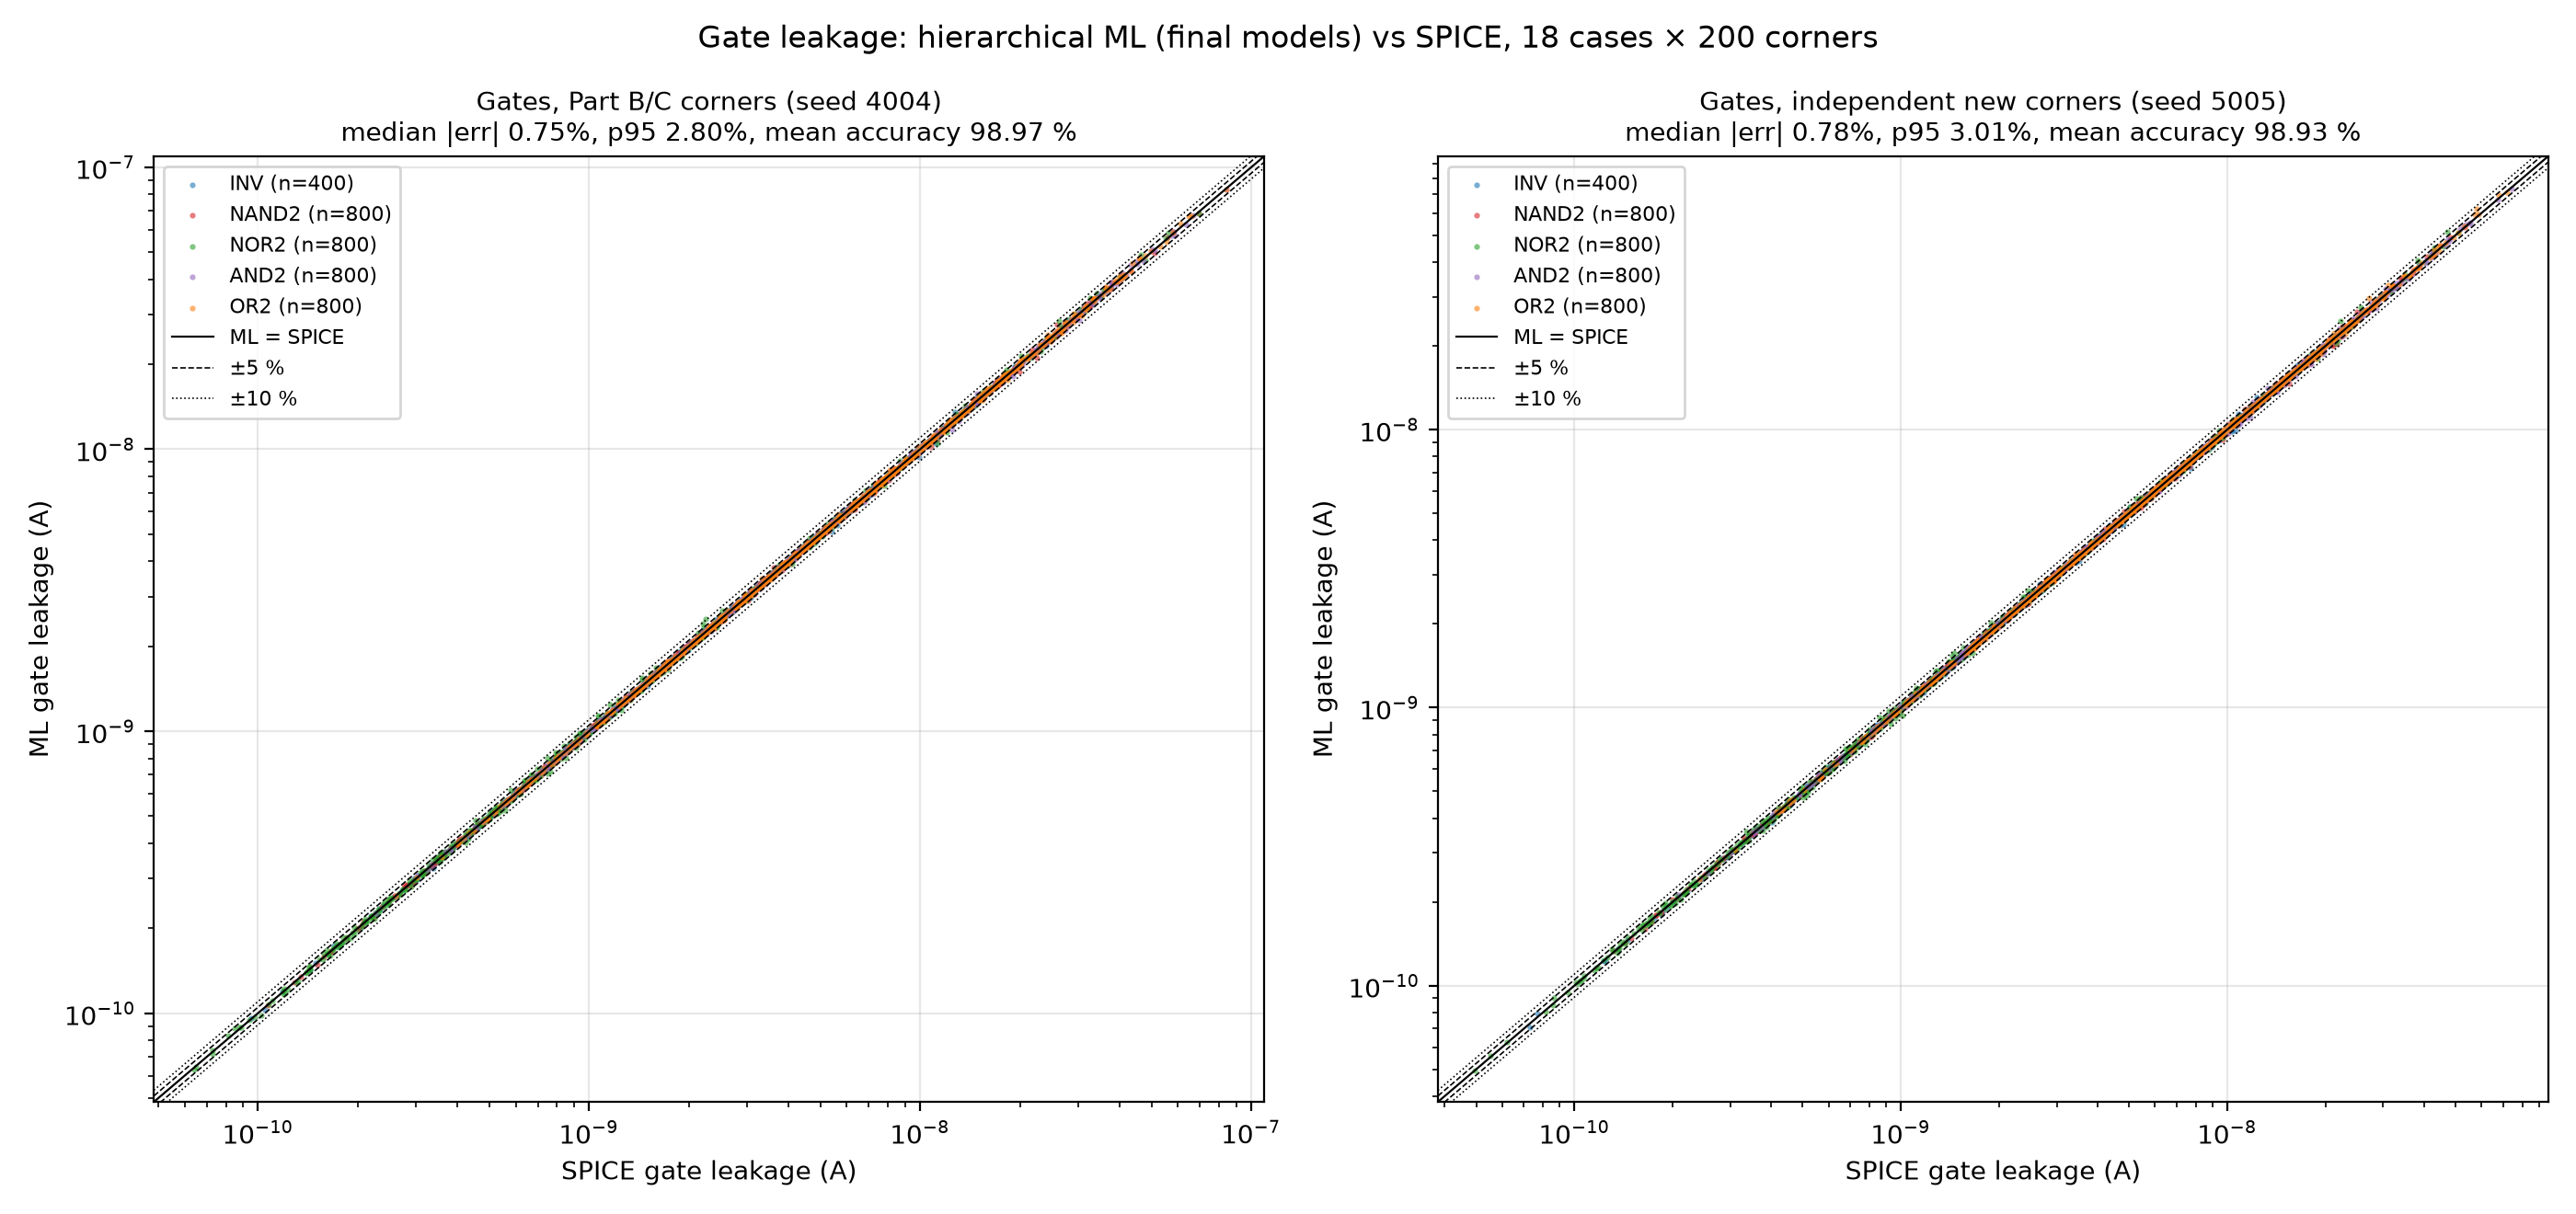
\includegraphics[width=\textwidth]{fig6_gate_parity.png}
\caption{Gate parity plot on log axes: ML vs SPICE leakage for all gate simulations (left: Part B corners;
right: independent new corners). Dashed/dotted lines: $\pm5\pct$ / $\pm10\pct$.}
\end{figure}

\begin{figure}[H]
\centering
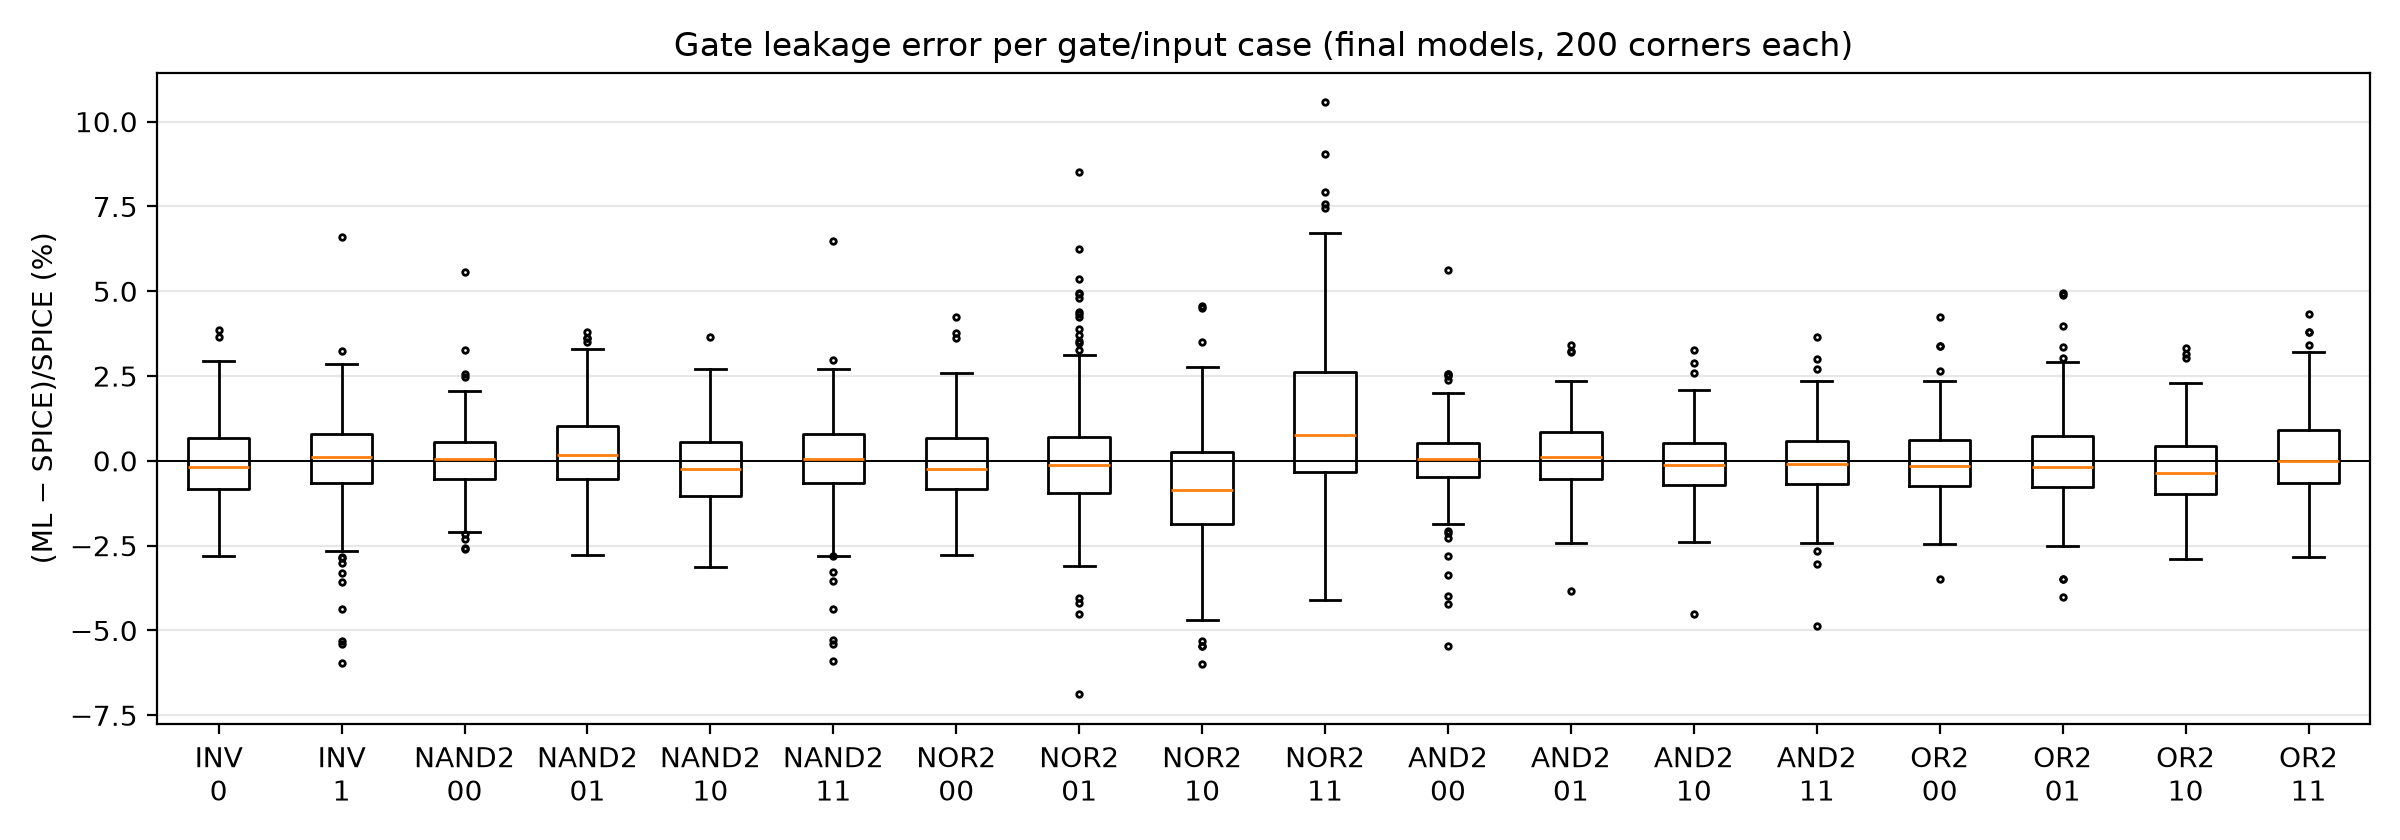
\includegraphics[width=\textwidth]{fig7_gate_error_by_case.png}
\caption{Signed error per gate/input case (200 corners each).}
\end{figure}

% ------------------------------------------------------------------------------------------
\section{Test circuit: 3-bit carry-lookahead adder}
\subsection{Design}
$G_i = A_i B_i$, $P_i = A_i \oplus B_i$, $C_1 = G_0 + P_0 C_0$, $C_2 = G_1 + P_1 G_0 + P_1 P_0 C_0$,
$C_3 = G_2 + P_2 G_1 + P_2 P_1 G_0 + P_2 P_1 P_0 C_0$ (carry-out), $S_i = P_i \oplus C_i$, with $C_0 = C_\text{in}$.
Every carry is computed directly from $G/P/C_0$ (lookahead, no ripple; verified). Multi-input terms are trees
of 2-input gates, and XOR is built as AND2(OR2, NAND2), with NAND2$(A_i, B_i)$ shared with $G_i$ =
INV(NAND2). The circuit has 36 gates (15 AND2, 12 OR2, 6 NAND2, 3 INV) and 192 transistors, with the same
sizing, bodies and model cards as the gates.

\begin{figure}[H]
\centering
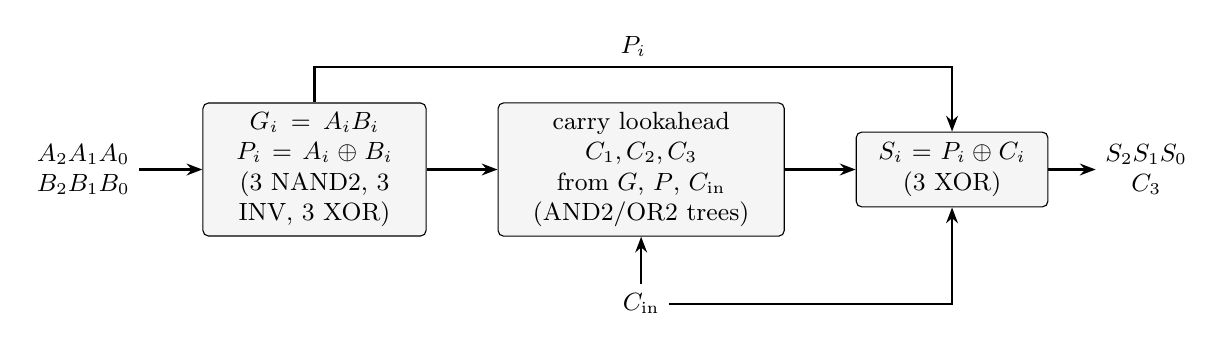
\begin{tikzpicture}[
  blk/.style={draw, rounded corners=2pt, align=center, font=\small, minimum height=0.95cm, fill=gray!8},
  arr/.style={-{Stealth[length=2mm]}, thick}, font=\small]
\node (in) [align=center] {$A_2A_1A_0$\\$B_2B_1B_0$};
\node[blk, right=0.8cm of in, text width=2.6cm] (gp) {$G_i = A_iB_i$\\$P_i = A_i \oplus B_i$\\(3 NAND2, 3 INV, 3 XOR)};
\node[blk, right=0.9cm of gp, text width=3.4cm] (cl) {carry lookahead\\$C_1, C_2, C_3$ from $G$, $P$, $C_\text{in}$\\(AND2/OR2 trees)};
\node[blk, right=0.9cm of cl, text width=2.2cm] (sum) {$S_i = P_i \oplus C_i$\\(3 XOR)};
\node (cin) [below=0.6cm of cl] {$C_\text{in}$};
\node (out) [right=0.6cm of sum, align=center] {$S_2S_1S_0$\\$C_3$};
\draw[arr] (in) -- (gp); \draw[arr] (gp) -- (cl); \draw[arr] (cl) -- (sum); \draw[arr] (sum) -- (out);
\draw[arr] (cin) -- (cl);
\draw[arr] (cin.east) -| (sum.south);
\draw[arr] (gp.north) -- ++(0,0.45) -| node[pos=0.25,above]{$P_i$} (sum.north);
\end{tikzpicture}
\caption{Structure of the 3-bit CLA built only from the five characterised gates.}
\end{figure}

All seven inputs ($A_2..A_0$, $B_2..B_0$, $C_\text{in}$) are driven at exactly 0 or VDD, so every input
combination is $2^7 = 128$ vectors (vector id $= A + 8B + 64C_\text{in}$); the Boolean model is verified
exhaustively. The $C_\text{in} = 0$ half was simulated first and the $C_\text{in} = 1$ half was added later with
the same netlist generator, corners and options (Fig.~\ref{fig:screen-cla}).

\subsection{SPICE reference and ML prediction}
Full-circuit SPICE at the 200 Part B corners: 25{,}600 runs, 0 failed. In every run the outputs equal
$A + B + C_\text{in}$ and all 36 internal nets are at their logic levels. For the ML prediction, a Boolean
simulation gives each gate's inputs; each gate's leakage is the gate model above for that gate type, input
pattern and corner; the circuit leakage is the sum over the 36 gates. No full-circuit SPICE quantity is used.

\begin{figure}[H]
\centering
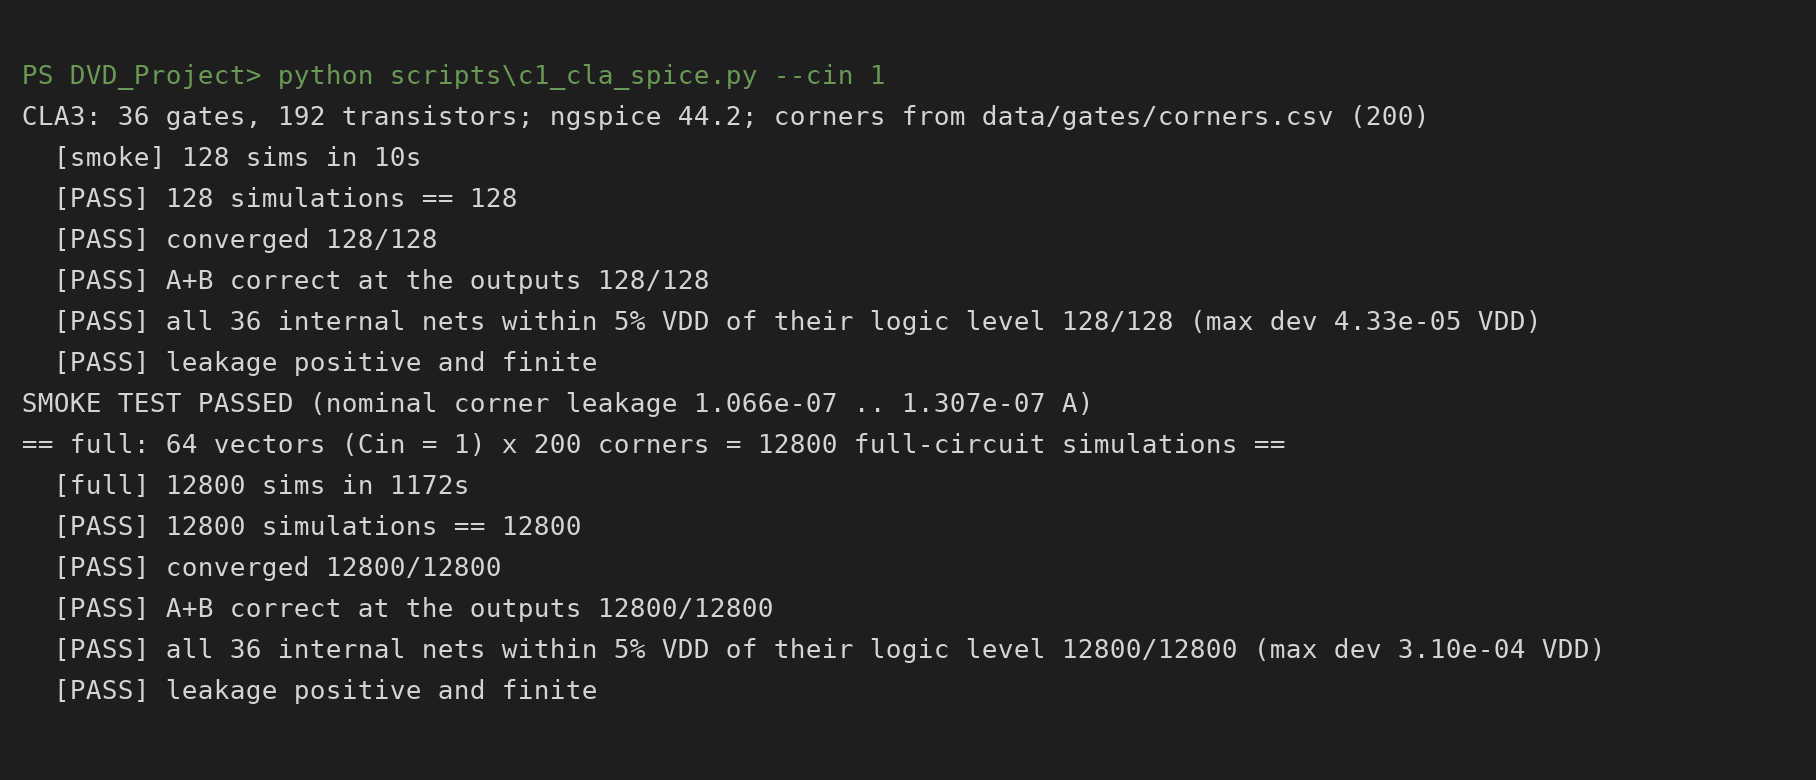
\includegraphics[width=0.92\textwidth]{screen_cla_cin1.png}
\caption{Screenshot: full-circuit SPICE run of the $C_\text{in} = 1$ half (12{,}800 simulations) with its
automatic checks.}
\label{fig:screen-cla}
\end{figure}

\subsection{Results}
\begin{table}[H]
\centering
\caption{3-bit CLA: hierarchical ML vs full-circuit SPICE, all 128 input combinations $\times$ 200 corners
($n = 25{,}600$ per corner set).}
\small\setlength{\tabcolsep}{4pt}
\begin{tabular}{lccccccc}
\toprule
Corner set & SPICE median (A) & ML median (A) & Bias & Median & p95 & $R^2(\log_{10})$ & Mean acc. \\
\midrule
Part B corners & 1.939e-07 & 1.935e-07 & $-0.093$\pct & 0.57\pct & 1.83\pct & 0.99992 & 99.29\pct \\
New corners & 1.997e-07 & 2.002e-07 & $+0.099$\pct & 0.58\pct & 2.25\pct & 0.99988 & \textbf{99.22\pct} \\
\bottomrule
\end{tabular}
\end{table}

\begin{table}[H]
\centering
\caption{CLA results split by carry-in.}
\begin{tabular}{llccccc}
\toprule
Corner set & Subset & $n$ & Bias & Median err & p95 err & Mean accuracy \\
\midrule
Part B corners & $C_\text{in} = 0$ & 12{,}800 & $-0.106$\pct & 0.57\pct & 1.81\pct & 99.30\pct \\
Part B corners & $C_\text{in} = 1$ & 12{,}800 & $-0.078$\pct & 0.58\pct & 1.86\pct & 99.28\pct \\
New corners & $C_\text{in} = 0$ & 12{,}800 & $+0.085$\pct & 0.57\pct & 2.26\pct & 99.24\pct \\
New corners & $C_\text{in} = 1$ & 12{,}800 & $+0.111$\pct & 0.59\pct & 2.23\pct & 99.20\pct \\
\bottomrule
\end{tabular}
\end{table}

\begin{figure}[H]
\centering
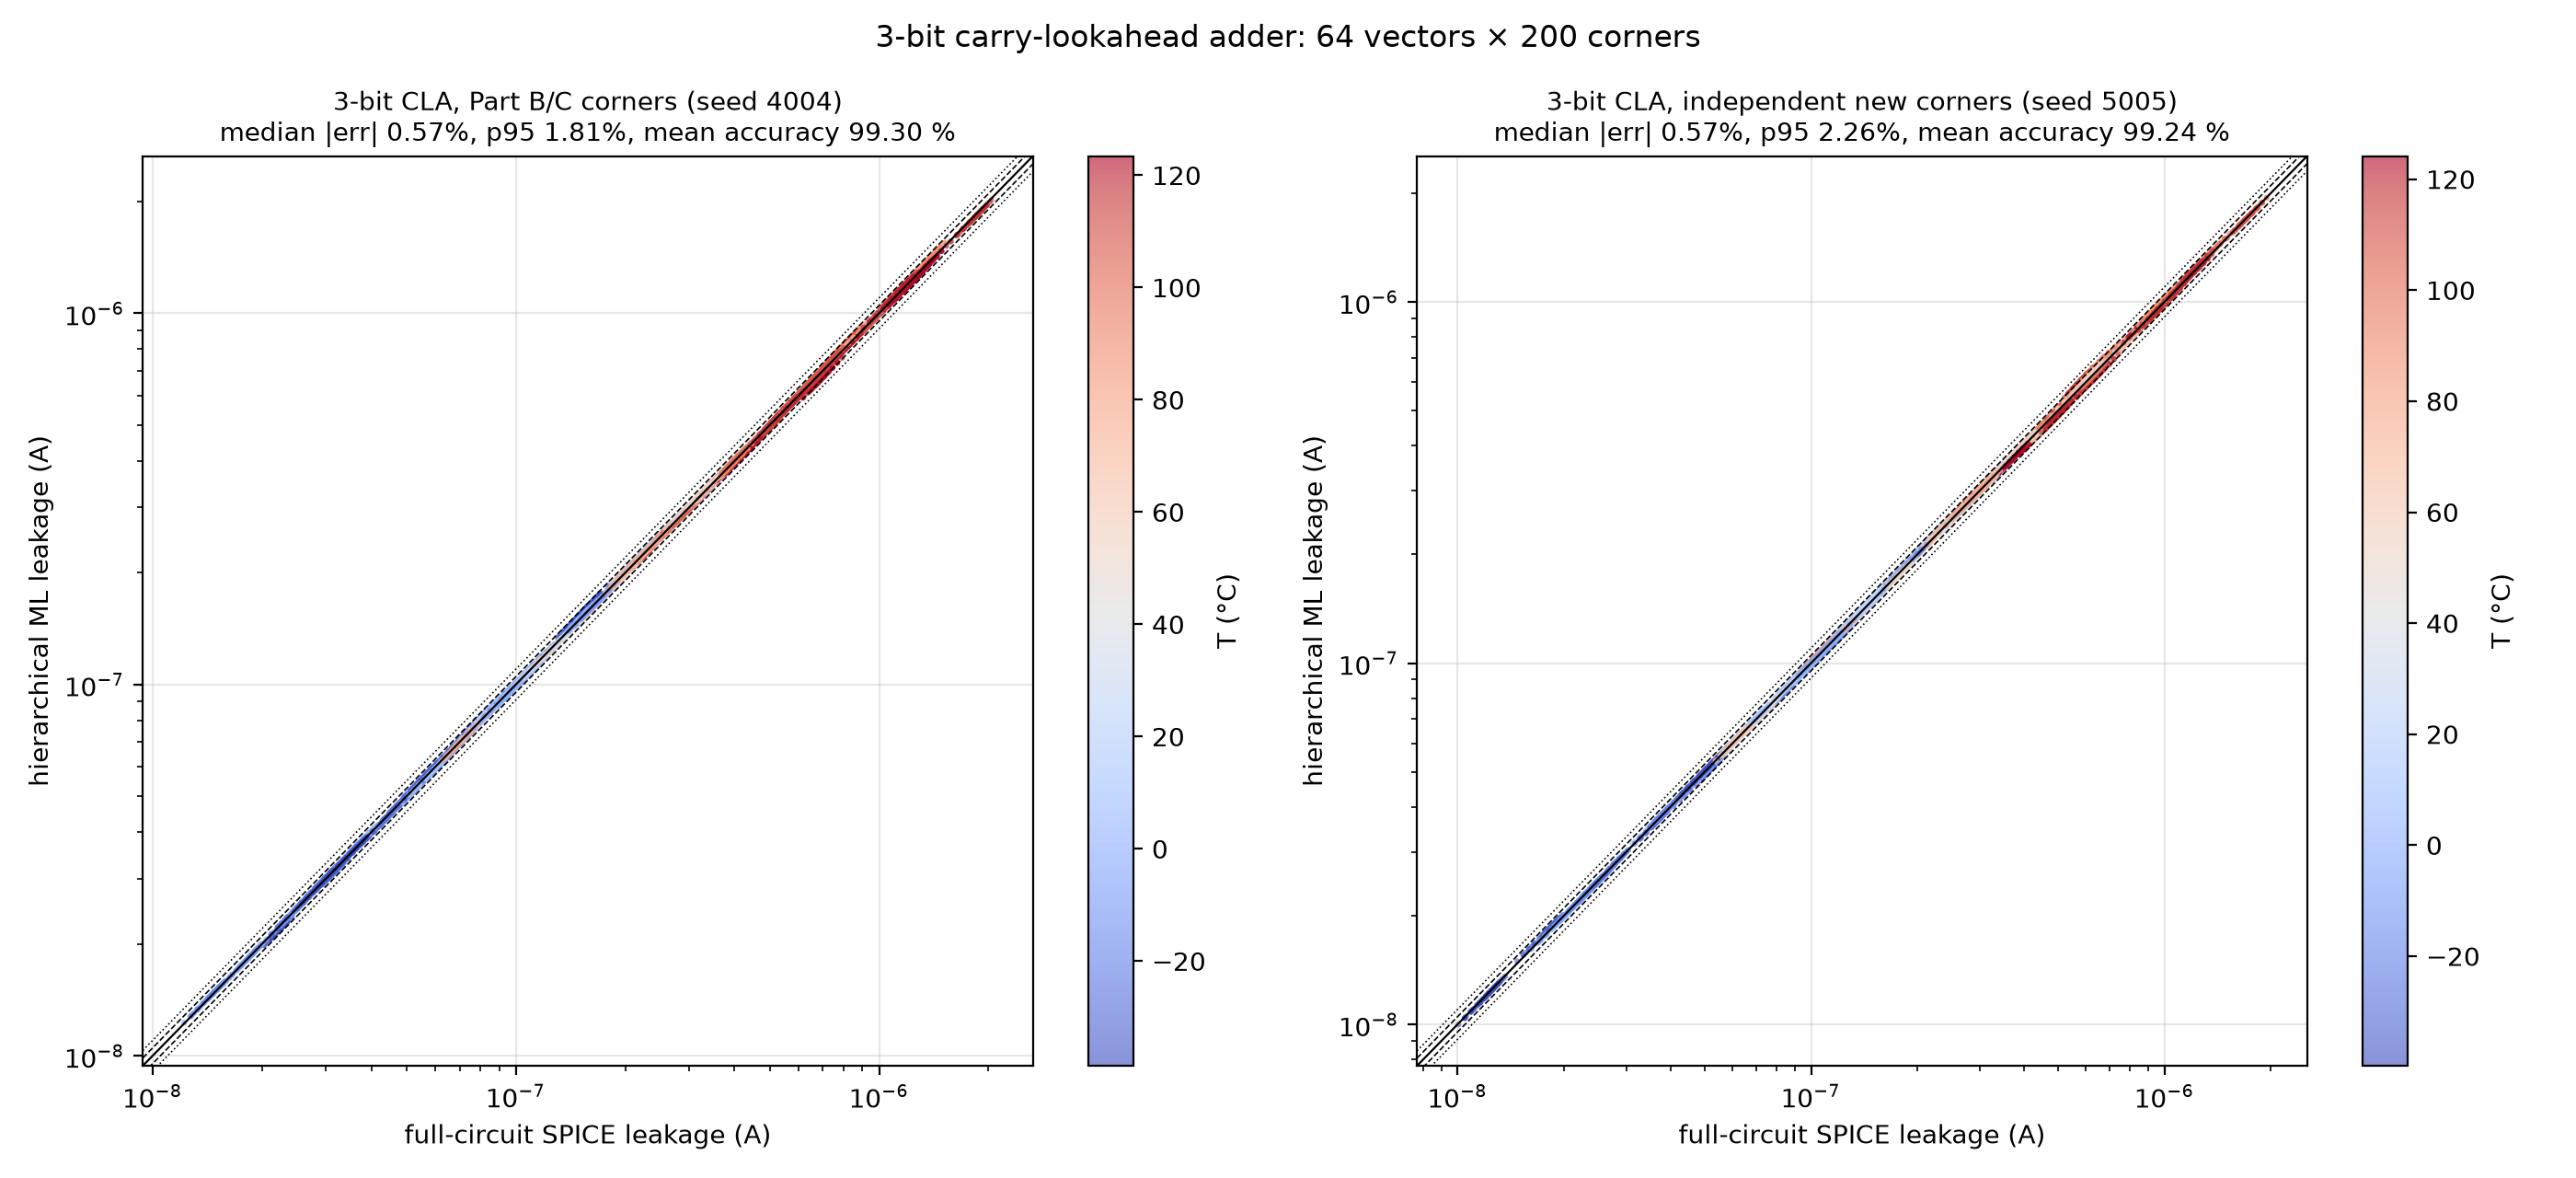
\includegraphics[width=\textwidth]{fig8_cla3_parity.png}
\caption{CLA parity plot on log axes, coloured by temperature (left: Part B corners; right: new corners).}
\end{figure}

\textbf{Comparison with gate-level accuracy.} The specification expects the circuit to be somewhat less
accurate than the gates because loading between gates is ignored. We measured the size of that effect
directly: summing the isolated-gate SPICE leakages (no ML) reproduces the full-circuit SPICE leakage with a
median error of 0.0062\pct\ (p95 0.046\pct) at the Part B corners and 0.0068\pct\ (p95 0.049\pct) at the new
corners, so loading is negligible at leakage-level currents and the circuit error is the transistor-ML error.
The circuit is in fact \emph{more} accurate than a single gate (median 0.58\pct\ vs 0.78\pct\ on the new
corners) because the errors of the 36 gates have different signs and partly cancel in the sum.

% ------------------------------------------------------------------------------------------
\section{Error analysis}
\textbf{Transistor level.} $I_g$ and $I_b$ are the easiest terminals (median 0.16--0.47\pct); $I_d$/$I_s$ carry
most of the error (median 0.67--1.16\pct). The largest errors are for ON devices at small $|V_{ds}|$ and for OFF
devices where the channel and gate-to-drain currents nearly cancel, where zero crossings make relative errors
unbounded. Optimisation was the dominant limit of the earlier models (iteration cap); after it was removed,
coverage of the near-rail region became the limit, partly fixed with extra targeted data.

\textbf{Gate level.} For every transistor instance the device-power error $|P_\text{ML} - P_\text{SPICE}|$ was
computed against the SPICE transistor currents of the same gate run (final models, all 3{,}600 Part B
samples). OFF transistors account for 88.3\pct\ of the summed device-power error, and the device with the
largest error is an OFF transistor in 85.4\pct\ of the samples; 89.4\pct\ of the OFF-device error comes from OFF
devices with (nearly) the full supply across them ($|V_{ds}| \ge 0.9\,$VDD). In the three least accurate cases
(all NOR2) the device that most often has the largest error is a wide series PMOS ($W = 360$\,nm, OFF): NOR2 11
\code{mpb} (95\pct\ of corners), NOR2 10 \code{mpa} (56\pct), NOR2 01 \code{mpb} (88\pct).

\textbf{Corner conditions.} The error grows with temperature:
\begin{table}[H]
\centering
\caption{Signed gate error vs temperature (final models, Part B corners).}
\begin{tabular}{lcc}
\toprule
Temperature & Bias (median signed error) & Median $|$error$|$ \\
\midrule
$-40$ to 15\,$^\circ$C & $-0.03$\pct & 0.67\pct \\
15 to 70\,$^\circ$C & $-0.11$\pct & 0.75\pct \\
70 to 125\,$^\circ$C & $-0.07$\pct & 0.88\pct \\
\bottomrule
\end{tabular}
\end{table}

\begin{figure}[H]
\centering
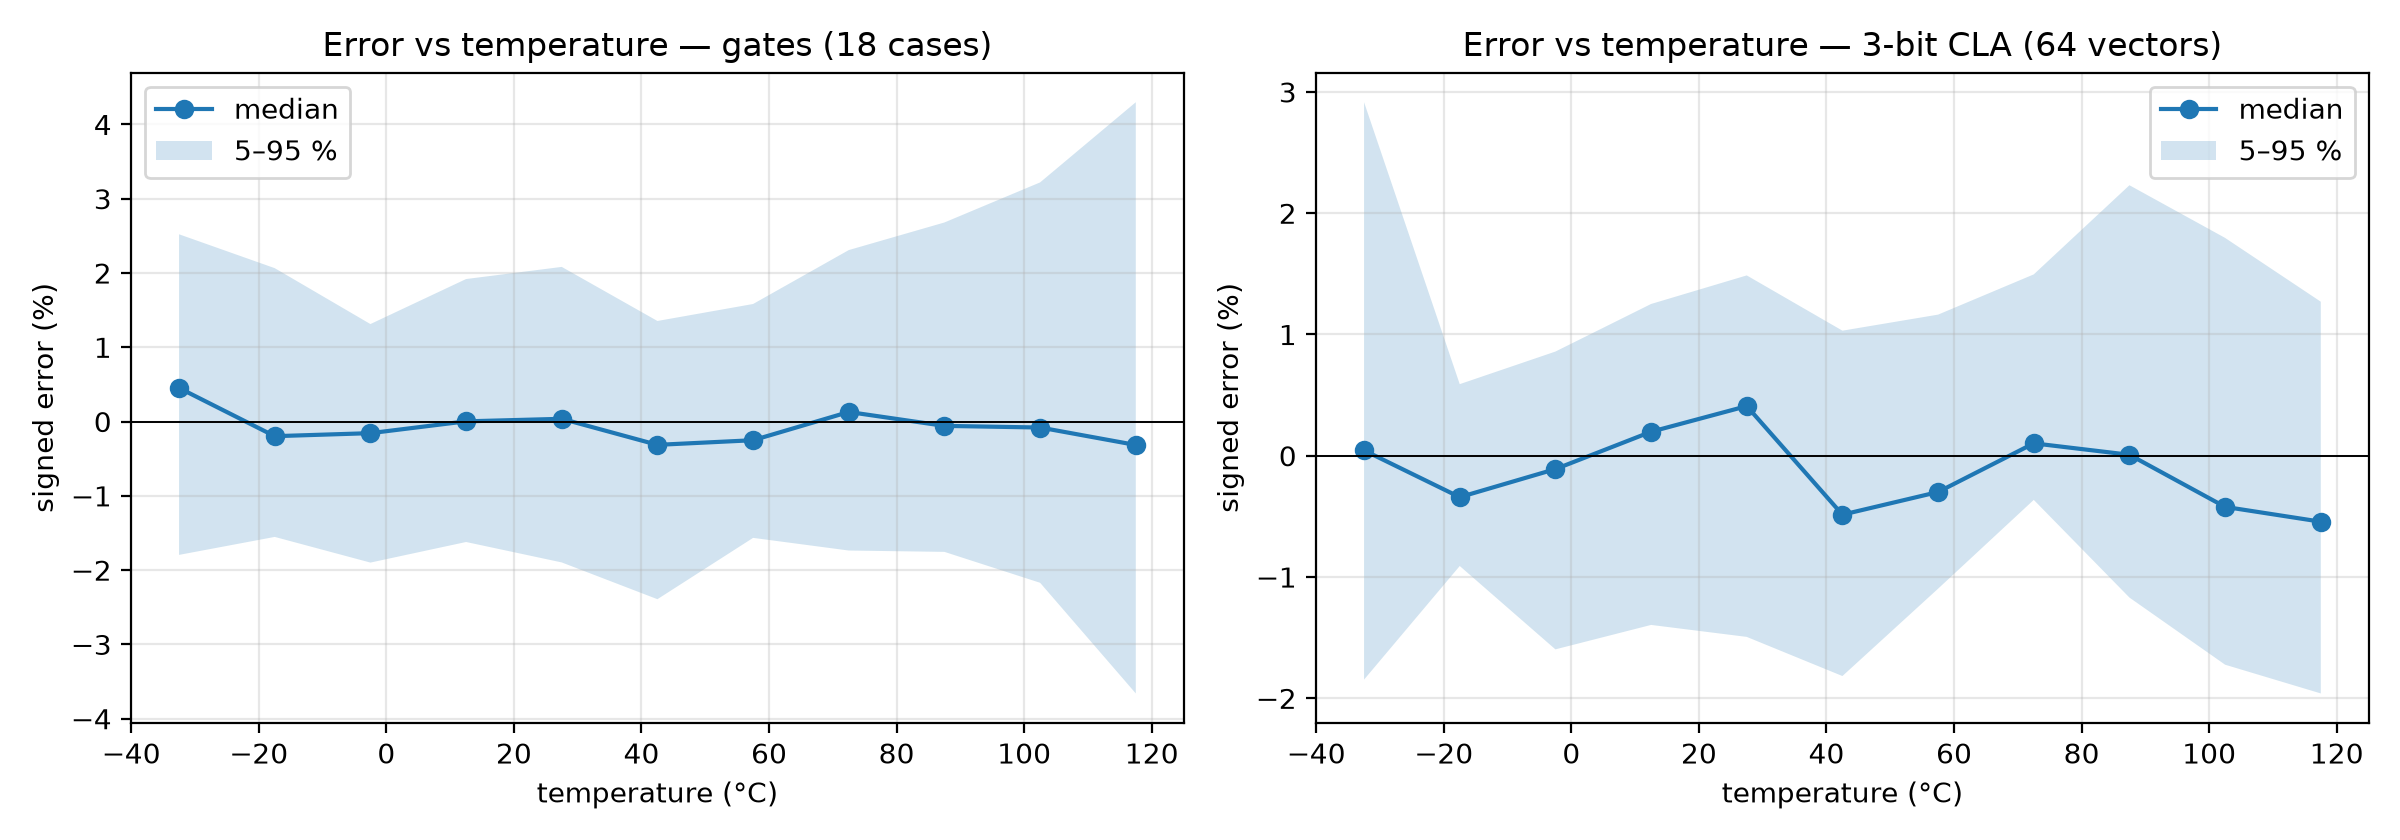
\includegraphics[width=\textwidth]{fig9_error_vs_temperature.png}
\caption{Signed error vs temperature for the gates and the CLA (median and 5--95\pct\ band).}
\end{figure}

\textbf{SPICE reference integrity.} One new-corner gate record (AND2 00, corner 83) had a spurious operating
point: with \code{rbodymod = 1} ngspice's default solve converged to a non-physical internal body-node state
(1.07e-8\,A instead of 5.28e-10\,A). Re-solving every reference with gmin stepping from the start (SPICE only,
no ML) flagged only this record out of 7{,}200 gate and 51{,}200 CLA references. It is corrected in a separate
file (the original is kept); the corrected value is the solution whose transistors match isolated
single-transistor SPICE.

\textbf{Before vs after the improvement phase} (independent new corners; CLA rows are the $C_\text{in} = 0$
half, evaluated before the $C_\text{in} = 1$ half existed): gate mean accuracy 95.12\pct\ $\to$ 98.93\pct\
(median 3.80\pct\ $\to$ 0.78\pct); CLA 96.25\pct\ $\to$ 99.24\pct\ (median 2.98\pct\ $\to$ 0.57\pct).

\begin{figure}[H]
\centering
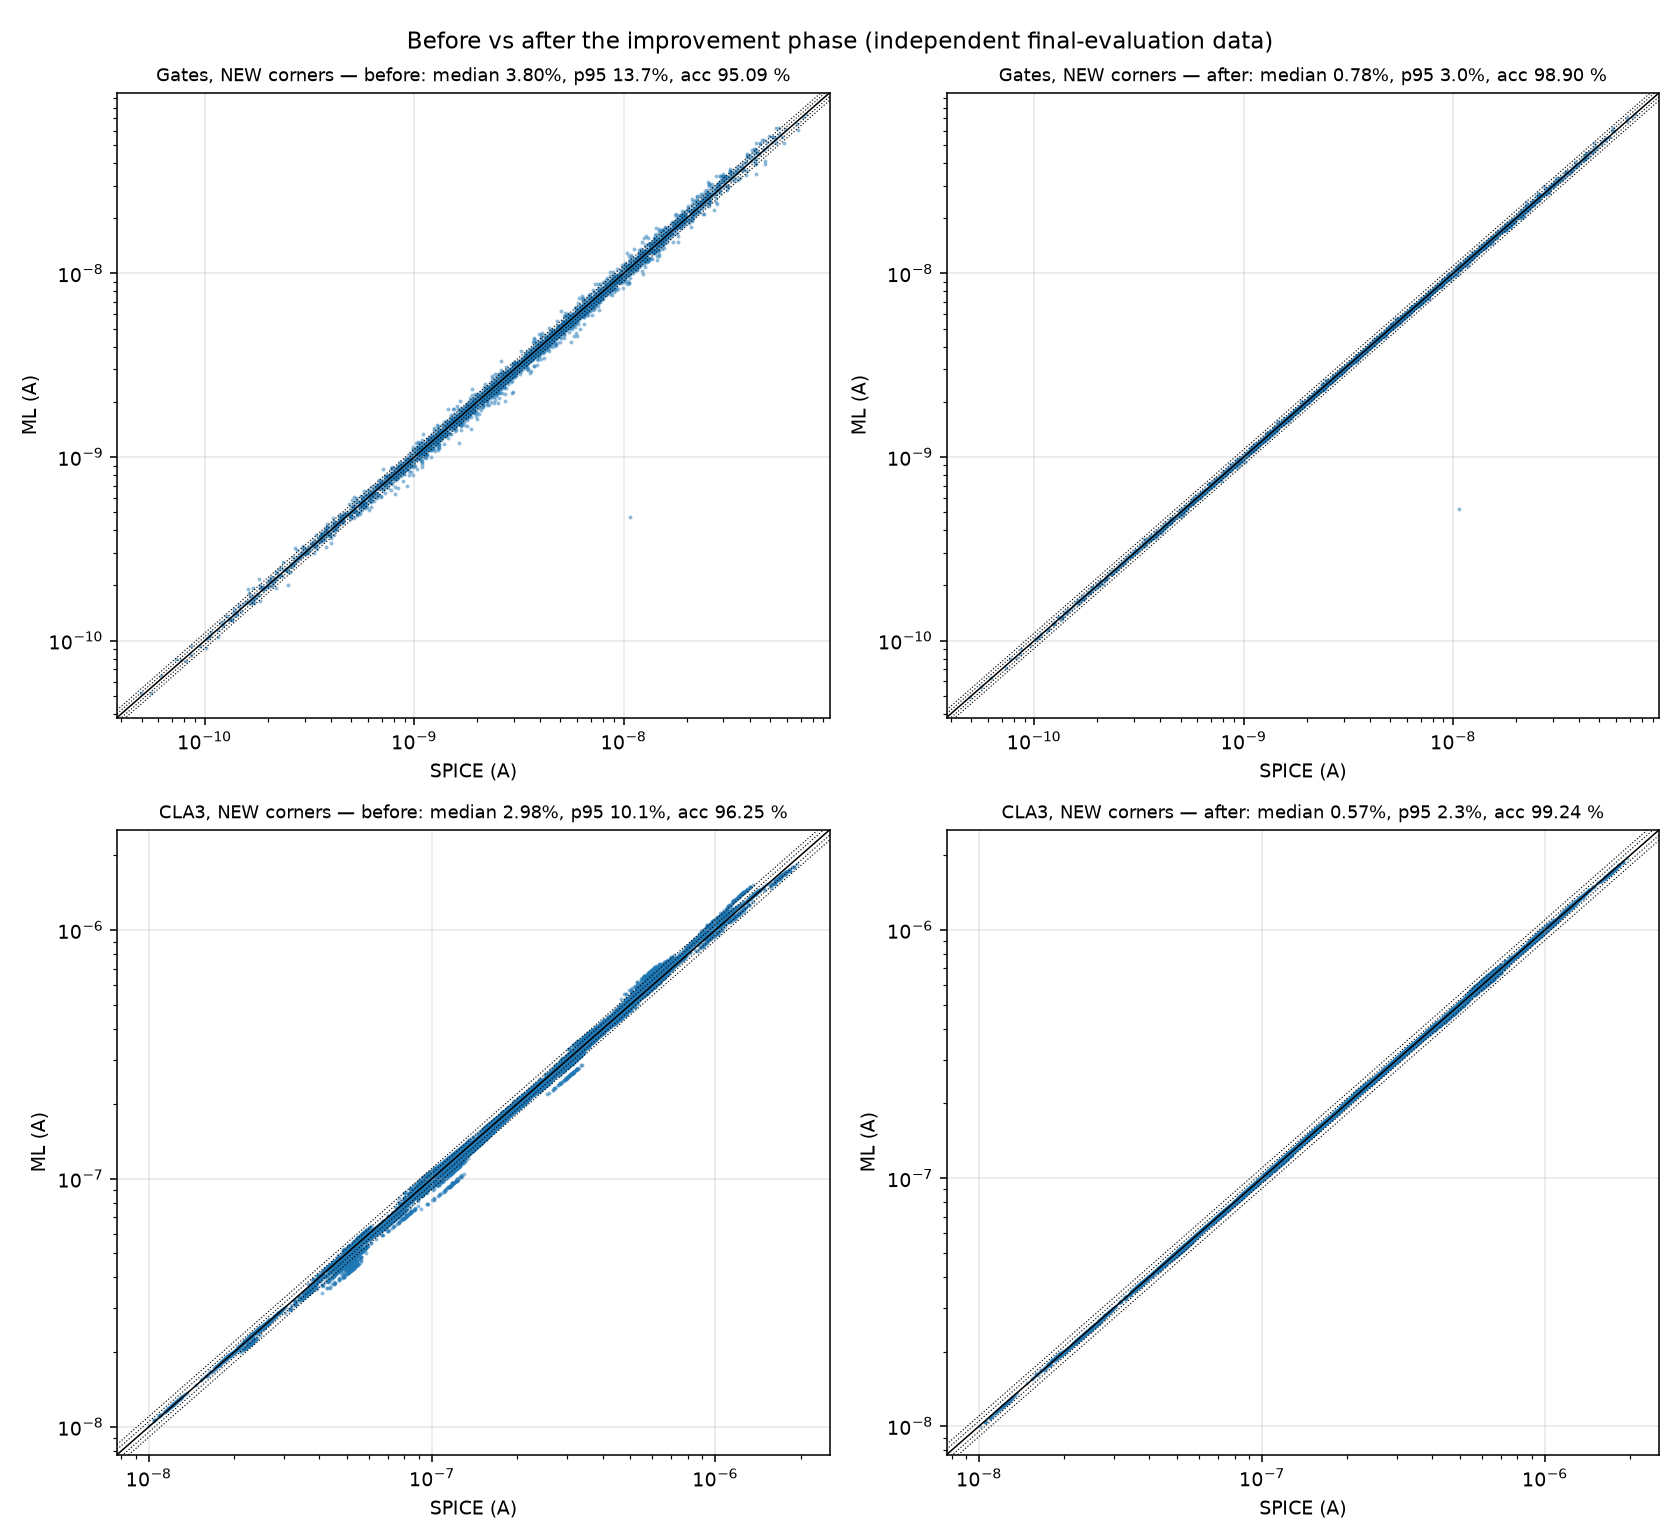
\includegraphics[width=\textwidth]{fig11_before_after.png}
\caption{Parity before and after the improvement phase.}
\end{figure}

% ------------------------------------------------------------------------------------------
\section{Limitations and improvements}
\begin{itemize}
\item Mean accuracy on independent data: circuit 99.22\pct, gates 98.93\pct, transistors 98.56\pct; the 99\pct\
target is met at circuit level only. Longer training (some fits still hit the iteration cap), larger seed
ensembles and more near-rail data would likely help; each MLP fit costs 1--2\,h of CPU time.
\item Gate (and therefore circuit) prediction uses SPICE-recorded internal node voltages, as the
specification allows. A fully SPICE-free flow would need a node-voltage model, e.g.\ solving KCL at the internal
nodes with the transistor models.
\item Model assumptions inherited from the specification: only \code{toxe} varies (BSIM4 keeps \code{toxp}
nominal); no junction area/perimeter (body leakage $\sim$1e-14\,A, not proportional to $W$); the gate widths are
our choice (equal-drive sizing).
\item Relative error is ill-defined for currents that cross zero; tail statistics on near-rail data should be
read with that in mind.
\item Non-unique SPICE operating points (internal body nodes) can corrupt references silently; an
operating-point uniqueness check should be part of every reference generation.
\end{itemize}

\section{Conclusion}
A hierarchical, physics-aware ML flow estimates PVT-dependent leakage from transistor to circuit level.
Fitted on 49{,}600 single-transistor SPICE samples (of 64{,}000 simulated), it predicts the 3-bit CLA adder's
leakage on unseen PVT corners with 0.58\pct\ median error and \textbf{99.22\pct} mean accuracy over all 128 input
combinations, and individual gates with 98.93\pct, with no SPICE run at prediction time (the gate-internal node
voltages come from the gate-level SPICE references). The decisive factors were the signed-log target,
power-based (Tellegen) gate accounting, fully converged network training, targeted data near the rails, and
SPICE reference integrity checks.

\section*{Reproducibility}
\begin{figure}[H]
\centering
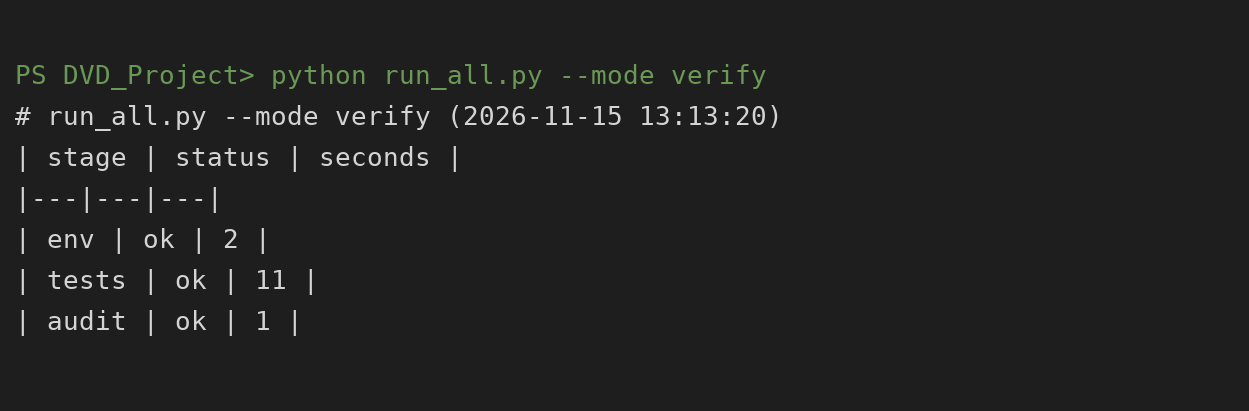
\includegraphics[width=0.55\textwidth]{screen_verify.png}
\caption{Screenshot: \code{run\_all.py -{}-mode verify} summary (environment check, 92 tests, deliverables audit).}
\end{figure}
Repository: \url{https://github.com/realsvira/DVD_Project}. The file
\path{reports/deliverables_checklist.md} maps every deliverable of the specification to its files.

\begin{thebibliography}{9}
\bibitem{spec} Course project specification, \emph{ML-Driven PVT Variation Aware Leakage Estimation}
(\code{DVD\_ML\_PROJECT.pdf}).
\bibitem{slides} Course slides, \emph{Project-1: Leakage estimation} (annotated), Z.~Abbas.
\bibitem{ptm} Predictive Technology Model (PTM), Arizona State University: 45\,nm high-performance metal-gate /
high-k model card.
\bibitem{bsim} BSIM4 MOSFET Model, User's Manual, BSIM Group, University of California, Berkeley.
\bibitem{ngspice} ngspice User's Manual, version 44.
\bibitem{sklearn} F.~Pedregosa et al., ``Scikit-learn: Machine Learning in Python,'' \emph{JMLR}, vol.~12,
pp.~2825--2830, 2011.
\bibitem{torch} A.~Paszke et al., ``PyTorch: An Imperative Style, High-Performance Deep Learning Library,''
\emph{NeurIPS}, 2019.
\bibitem{lgbm} G.~Ke et al., ``LightGBM: A Highly Efficient Gradient Boosting Decision Tree,'' \emph{NeurIPS}, 2017.
\bibitem{lbfgs} D.~C.~Liu and J.~Nocedal, ``On the limited memory BFGS method for large scale optimization,''
\emph{Mathematical Programming}, vol.~45, pp.~503--528, 1989.
\end{thebibliography}

\end{document}
